\documentclass[11pt,letterpaper]{article}
\usepackage[margin=1in]{geometry}
\usepackage{amsmath,amssymb,amsfonts}
\usepackage{mathtools}
\usepackage{booktabs}
\usepackage{graphicx}
\usepackage{xcolor}
\usepackage{hyperref}
\usepackage{enumitem}
\usepackage{caption}
\usepackage{float}
\usepackage{fancyhdr}
\usepackage{titlesec}
\usepackage{subcaption}

\hypersetup{colorlinks=true, linkcolor=blue!60!black, citecolor=blue!60!black, urlcolor=blue!60!black}

\definecolor{ansatzblue}{RGB}{31,119,180}
\definecolor{residred}{RGB}{214,39,40}
\definecolor{spingreen}{RGB}{44,160,44}

\pagestyle{fancy}
\fancyhf{}
\rhead{\small\textit{Modulation Interpretability}}
\lhead{\small\textit{Islam et al.}}
\cfoot{\thepage}

\titleformat{\section}{\large\bfseries}{\thesection}{1em}{}
\titleformat{\subsection}{\normalsize\bfseries}{\thesubsection}{1em}{}

\newcommand{\xamp}{\xi_{\rm amp}}
\newcommand{\xomg}{\xi_{\omega}}
\newcommand{\dxamp}{\delta\xi_{\rm amp}}
\newcommand{\dxomg}{\delta\xi_{\omega}}
\newcommand{\chiS}{\chi_S}
\newcommand{\chiA}{\chi_A}
\newcommand{\calE}{\mathcal{E}}

\begin{document}

\begin{center}
{\LARGE\bfseries Interpreting the Fitted Analytic\\[4pt] Eccentric Modulation Formula}\\[12pt]
{\large Structural analysis, post-Newtonian comparison, and compactification}\\[8pt]
{\normalsize Modulation Learning Project --- Small-Spin Eccentric Study}\\[4pt]
{\small\today}
\end{center}

\vspace{6pt}
\hrule
\vspace{12pt}

\tableofcontents
\vspace{12pt}
\hrule
\vspace{12pt}

%======================================================================
\section{Overview}
%======================================================================

We have constructed an analytic model for the eccentric gravitational-wave modulation functions $\xamp(t)$ and $\xomg(t)$ for the dominant $(2,2)$ mode of spinning binary black holes. The model combines a known post-Newtonian (PN) ansatz with a data-driven Ridge regression correction, achieving waveform accuracy $\calE = 4.2 \times 10^{-4}$ (median) across the parameter space
\begin{equation}
q \in [1,10], \quad |\chi_{1,2}| \leq 0.5, \quad e_0 \in [0.001, 0.5]\,.
\end{equation}

This document analyzes the structure of the 2955-term fitted expression, identifies its connection to known PN expressions, and proposes strategies for compactifying it into a closed-form representation.

%======================================================================
\section{Total Modulation Decomposition}
%======================================================================

The eccentric waveform is reconstructed from a quasi-circular baseline via
\begin{align}
A_{\rm pred}(t) &= A_{\rm cir}(t)\,\bigl(1 + \xamp(t)\bigr)\,, \label{eq:Apred}\\
\omega_{\rm pred}(t) &= \omega_{\rm cir}(t)\,\bigl(1 + \xomg(t)\bigr)\,, \label{eq:wpred}\\
\phi_{\rm pred}(t) &= \int \omega_{\rm pred}\,dt\,, \label{eq:phipred}\\
h_{22}^{\rm pred}(t) &= A_{\rm pred}\,e^{i\phi_{\rm pred}}\,. \label{eq:hpred}
\end{align}

Each modulation function is decomposed as an analytically known \textbf{ansatz} plus a data-driven \textbf{residual}:
\begin{equation}
\boxed{\xamp(t) = \underbrace{\bigl|\,h_{22}^{\rm ecc}(x, e, \zeta, \nu)\bigr| - 1}_{\text{PN ansatz (0PN + 1PN)}} \;+\; \underbrace{\dxamp(e, x, \zeta, \nu, \chiS, \chiA)}_{\text{Ridge residual (2955 terms)}}}
\label{eq:decomp}
\end{equation}
and similarly for $\xomg$, with ansatz $\xomg^{\rm ansatz} = \xamp^{\rm ansatz}/0.9$ from gwNRXHME Relation~III.

%======================================================================
\section{The PN Ansatz: \texorpdfstring{$h_{22}^{\rm ecc}$}{h22ecc} from hFactEccCorr[2,2]}
\label{sec:ansatz}
%======================================================================

\subsection{Origin}

The ansatz is the $(2,2)$ eccentric correction factor \texttt{hFactEccCorr[2,2]} from Gamboa, Khalil \& Buonanno (\texttt{EOB\_modes.dat.m}, lines 13233--13812). The full expression contains PN orders through 2.5PN; our implementation uses the \textbf{0PN + 1PN truncation}:

\begin{equation}
h_{22}^{\rm ecc}(x, e, \zeta, \nu) = \underbrace{\frac{4 + 2e^2\,e^{2i\zeta} + e\,e^{-i\zeta} + 5e\,e^{i\zeta}}{4(1 - e^2)}}_{\displaystyle\text{0PN (Newtonian)}} \;+\; \underbrace{\frac{x\,e}{(1 - e^2)^2}\;\mathcal{C}(\zeta, e, \nu)}_{\displaystyle\text{1PN correction}}
\label{eq:ansatz}
\end{equation}

where the 1PN curly bracket contains Fourier modes $e^{ik\zeta}$ for $k \in \{-3, \ldots, +3\}$:
\begin{align}
\mathcal{C} &= e\Bigl(\tfrac{26\nu}{7} - \tfrac{559}{84}\Bigr) + e\,e^{-2i\zeta}\Bigl(\tfrac{15\nu}{14} - \tfrac{95}{168}\Bigr) + e^2\,e^{-3i\zeta}\Bigl(\tfrac{9\nu}{56} + \tfrac{1}{112}\Bigr) \nonumber\\
&\quad + e^2\,e^{3i\zeta}\Bigl(\tfrac{\nu}{8} - \tfrac{49}{48}\Bigr) + e^{2i\zeta}\Bigl[e^3\Bigl(\tfrac{6\nu}{7} - \tfrac{41}{21}\Bigr) + e\Bigl(\tfrac{\nu}{14} - \tfrac{153}{56}\Bigr)\Bigr] \nonumber\\
&\quad + e^{-i\zeta}\Bigl[e^2\Bigl(\tfrac{7\nu}{8} - \tfrac{59}{48}\Bigr) + \tfrac{27\nu}{14} - \tfrac{23}{14}\Bigr] + e^{i\zeta}\Bigl[e^2\Bigl(\tfrac{143\nu}{56} - \tfrac{2071}{336}\Bigr) + \tfrac{\nu}{14} - \tfrac{13}{7}\Bigr]\,.
\label{eq:curly}
\end{align}

\subsection{Fourier content of the ansatz}

A critical structural property: $\xamp^{\rm ansatz} = |h_{22}^{\rm ecc}| - 1$ contains \textbf{only} $\cos k\zeta$ harmonics --- the absolute value operation annihilates all $\sin k\zeta$ content. At representative values $e = 0.3$, $\nu = 0.25$:

\begin{table}[H]
\centering
\caption{Fourier decomposition of $\xamp^{\rm ansatz}$ at $e = 0.3$, $\nu = 0.25$, for different PN orders ($x$ values).}
\label{tab:ansatz_fourier}
\begin{tabular}{@{}lcccc@{}}
\toprule
& $c_0$ (mean) & $\cos\zeta$ & $\cos 2\zeta$ & $\sin k\zeta$ \\
\midrule
0PN ($x = 0$) & $+0.124$ & $+0.497$ & $+0.025$ & $\equiv 0$ \\
0PN + 1PN ($x = 0.05$) & $+0.091$ & $+0.431$ & $+0.010$ & $\equiv 0$ \\
0PN + 1PN ($x = 0.10$) & $+0.057$ & $+0.364$ & $-0.005$ & $\equiv 0$ \\
\bottomrule
\end{tabular}
\end{table}

\noindent The $\cos\zeta$ harmonic dominates ($>80\%$ of the variance). The 1PN correction reduces the mean and fundamental amplitude, consistent with the relativistic shrinking of eccentricity during inspiral.

\subsection{Full PN structure in EOB\_modes.dat.m}

The complete \texttt{hFactEccCorr[2,2]} contains five PN orders:

\begin{table}[H]
\centering
\caption{PN hierarchy of hFactEccCorr[2,2]. The implemented ansatz includes only the first two rows.}
\label{tab:pn_orders}
\begin{tabular}{@{}cccll@{}}
\toprule
PN order & $x$ power & Prefactor & Max $e$ power & Physics \\
\midrule
0PN & $x^0$ & $(1 - e^2)^{-1}$ & $e^2$ & Keplerian orbit \\
1PN & $x^1$ & $(1 - e^2)^{-2}$ & $e^3$ & First relativistic correction \\
\midrule
1.5PN & $x^{3/2}$ & $(1 - e^2)^{-7/2}$ & $e^8$ & Tail terms ($\pi$, $\log$) \\
2PN & $x^2$ & $(1 - e^2)^{-3}$ & $e^6$ & Second-order, $\nu^2$-dependent \\
2.5PN & $x^{5/2}$ & $(1 - e^2)^{-7/2}$ & $e^{10}$ & Higher tail \\
\bottomrule
\end{tabular}
\end{table}

\noindent The Ridge residual must absorb everything below the horizontal rule.

%======================================================================
\section{Structure of the Fitted Residual}
\label{sec:residual}
%======================================================================

\subsection{Basis specification}

The best model (\texttt{ridge\_nh7\_me5\_mchi1\_a1e-06}) uses the basis:
\begin{equation}
\dxamp = \sum_{g=1}^{197} e^{a_g}\, x^{b_g}\, \nu^{c_g}\, \chiS^{d_g}\, \chiA^{f_g} \left[\, c_0^{(g)} + \sum_{k=1}^{7} \bigl(\alpha_k^{(g)} \cos k\zeta + \beta_k^{(g)} \sin k\zeta\bigr) \right]
\label{eq:residual}
\end{equation}
with the constraint $a_g \geq 1$ (modulations vanish at $e = 0$) and total degree bound $a + b + c + d + f \leq 8$.

\begin{table}[H]
\centering
\caption{Basis parameters for the best Ridge model.}
\label{tab:basis}
\begin{tabular}{@{}lccl@{}}
\toprule
Parameter & Symbol & Range & Meaning \\
\midrule
\texttt{max\_e} & $a$ & $1$--$5$ & Eccentricity powers \\
\texttt{max\_x} & $b$ & $0$--$3$ & Frequency powers (0PN to 3PN) \\
\texttt{max\_nu} & $c$ & $0$--$2$ & Mass ratio powers \\
\texttt{max\_chi} & $d, f$ & $0$--$1$ & Spin powers ($\chiS$, $\chiA$) \\
\texttt{n\_harm} & $k$ & $1$--$7$ & Fourier harmonics in $\zeta$ \\
\midrule
\multicolumn{2}{l}{Power-law groups} & 197 & \\
\multicolumn{2}{l}{Features per group} & 15 & ($1 + 2 \times 7$) \\
\multicolumn{2}{l}{\textbf{Total coefficients}} & \textbf{2955} & (per modulation function) \\
\bottomrule
\end{tabular}
\end{table}

\subsection{Harmonic hierarchy}

\begin{table}[H]
\centering
\caption{Distribution of coefficient weight $\sum_g |\mathbf{c}^{(g)}|$ by Fourier harmonic number.}
\label{tab:harmonics}
\begin{tabular}{@{}crr@{}}
\toprule
Harmonic $k$ & Total $|\mathbf{c}|$ & Fraction \\
\midrule
$k = 0$ (base) & 350 & 8.6\% \\
$\mathbf{k = 1}$ & \textbf{2579} & \textbf{63.3\%} \\
$k = 2$ & 342 & 8.4\% \\
$k = 3$ & 124 & 3.0\% \\
$k = 4$ & 200 & 4.9\% \\
$k = 5$ & 120 & 2.9\% \\
$k = 6$ & 153 & 3.8\% \\
$k = 7$ & 190 & 4.7\% \\
\bottomrule
\end{tabular}
\end{table}

\noindent The $k = 1$ harmonic overwhelmingly dominates the residual. Crucially, this content is predominantly $\sin\zeta$ (not $\cos\zeta$), which is structurally absent from the ansatz (Section~\ref{sec:ansatz}).

\subsection{Eccentricity and PN order hierarchy}

\begin{table}[H]
\centering
\begin{minipage}[t]{0.45\textwidth}
\centering
\caption{Weight by eccentricity power.}
\label{tab:epow}
\begin{tabular}{@{}crr@{}}
\toprule
$e^a$ & $|\mathbf{c}|$ & Fraction \\
\midrule
$e^1$ & 2001 & 39.1\% \\
$e^2$ & 1467 & 28.7\% \\
$e^3$ & 788 & 15.4\% \\
$e^4$ & 507 & 9.9\% \\
$e^5$ & 346 & 6.8\% \\
\bottomrule
\end{tabular}
\end{minipage}
\hfill
\begin{minipage}[t]{0.45\textwidth}
\centering
\caption{Weight by PN order ($x$ power).}
\label{tab:xpow}
\begin{tabular}{@{}ccrr@{}}
\toprule
$x^b$ & PN & $|\mathbf{c}|$ & Fraction \\
\midrule
$x^0$ & 0PN & 1107 & 21.6\% \\
$x^1$ & 1PN & 2349 & 45.9\% \\
$x^2$ & 2PN & 1149 & 22.5\% \\
$x^3$ & 3PN & 503 & 9.8\% \\
\bottomrule
\end{tabular}
\end{minipage}
\end{table}

\noindent The 1PN sector ($x^1$) carries nearly half the residual weight. This is expected: the ansatz includes terms through 1PN, but with truncated eccentricity expansions and no $\sin\zeta$ content. The residual at 1PN fills both gaps.

\subsection{Spin sector decomposition}

\begin{table}[H]
\centering
\caption{Distribution of residual weight across spin sectors.}
\label{tab:spin}
\begin{tabular}{@{}lrrl@{}}
\toprule
Sector & Weight & Fraction & PN origin \\
\midrule
Non-spin ($\chiS^0 \chiA^0$) & 1890 & 36.9\% & 0PN--3PN (missing orders) \\
$\chiS$-linear & 1393 & 27.2\% & Spin-orbit (1.5PN) \\
$\chiA$-linear & 1390 & 27.2\% & Spin-orbit $\times\,\Delta$ (1.5PN) \\
$\chiS\,\chiA$ bilinear & 449 & 8.8\% & Spin-spin (2PN) \\
\bottomrule
\end{tabular}
\end{table}

\noindent \textbf{Key finding}: Spin corrections constitute \textbf{63\%} of the residual. This is the dominant new physics the residual captures, since the PN ansatz is entirely non-spinning. The near-equal $\chiS$ and $\chiA$ weights are consistent with the PN spin-orbit structure, where $\chiS$ and $\chiA\,\Delta$ enter symmetrically at 1.5PN.

%======================================================================
\section{Dominant Fitted Coefficients and PN Identification}
\label{sec:dominant}
%======================================================================

\subsection{Top 10 amplitude coefficients}

\begin{table}[H]
\centering
\caption{Ten largest coefficients of $\dxamp$ by magnitude. All dominant terms are $\sin\zeta$ harmonics.}
\label{tab:top10}
\begin{tabular}{@{}rlrrl@{}}
\toprule
Rank & Basis function & $c_{\rm amp}$ & $c_\omega$ & PN identification \\
\midrule
1 & $e^2\, x\, \nu\, \sin\zeta$ & $+100.7$ & $+135.5$ & 1PN $\times$ Im$(h_{22}^{\rm ecc})$ \\
2 & $e\, x^2\, \chiS\, \sin\zeta$ & $+90.6$ & $+139.8$ & Spin-orbit (1.5PN) \\
3 & $e\, x\, \nu\, \chiS\, \sin\zeta$ & $+79.5$ & $+113.3$ & Spin-orbit (1.5PN) \\
4 & $e\, x^2\, \chiA\, \sin\zeta$ & $+70.9$ & $+110.8$ & Spin-orbit $\times\,\Delta$ \\
5 & $e\, x\, \nu\, \chiA\, \sin\zeta$ & $+69.9$ & $+99.4$ & Spin-orbit $\times\,\Delta$ \\
6 & $e^2\, x^2\, \cos\zeta$ & $+61.3$ & $+69.1$ & 2PN correction \\
7 & $e^2\, x\, \chiS\, \sin\zeta$ & $+60.2$ & $+86.9$ & Spin-orbit, $e^2$-enhanced \\
8 & $e^3\, x\, \nu\, \sin\zeta$ & $+58.0$ & $+79.1$ & 1PN, higher ecc.\ order \\
9 & $e^2\, x\, \nu\, \cos\zeta$ & $-57.0$ & $-75.9$ & 1PN $\times$ Re correction \\
10 & $e^2\, x\, \chiA\, \sin\zeta$ & $+53.3$ & $+77.8$ & Spin-orbit $\times\,\Delta$, $e^2$ \\
\bottomrule
\end{tabular}
\end{table}

\subsection{Physical interpretation of the dominant terms}

\paragraph{(a) $\sin\zeta$ dominance.}
The five largest coefficients are all $\sin\zeta$ terms. This content arises because the ansatz uses $|h_{22}^{\rm ecc}| - 1$, which discards the complex phase. The imaginary part of the 0PN expression is:
\begin{equation}
\text{Im}\bigl(h_{22}^{\rm ecc}\bigr)\Big|_{\rm 0PN} \supset \frac{e\,(5 - 1)\sin\zeta}{4(1 - e^2)} = \frac{e\,\sin\zeta}{1 - e^2}\,,
\label{eq:imag0pn}
\end{equation}
which generates precisely the $e^a \sin\zeta$ structure that dominates the residual. Physically, this represents the \textbf{orbital phase modulation}: gravitational-wave phase advances faster near pericenter and slower near apocenter, creating a $\sin\zeta$ asymmetry in the instantaneous frequency.

\paragraph{(b) Spin-orbit terms.}
In PN theory, the leading spin-orbit correction to the $(2,2)$ mode enters at $O(x^{3/2})$:
\begin{equation}
\delta h_{22}^{\rm SO} \sim x^{3/2} \cdot e \cdot \bigl(\chiS\, f_S(\nu) + \chiA\,\Delta\, f_A(\nu)\bigr) \cdot (\text{Fourier in } \zeta)\,.
\label{eq:so}
\end{equation}
Since $x^{3/2}$ is not in the integer-power basis, the model approximates it via:
\begin{equation}
x^{3/2} \approx c_1\, x + c_2\, x^2 \qquad \text{over } x \in [0, 0.1]\,,
\label{eq:x32approx}
\end{equation}
explaining why the largest spin terms appear at \emph{both} $x^1$ (ranks 3, 5) and $x^2$ (ranks 2, 4). A half-integer power $x^{3/2}$ in the basis would consolidate these pairs.

\paragraph{(c) Higher eccentricity orders.}
The rank-8 term $e^3\, x\, \nu\, \sin\zeta$ represents 1PN corrections at $O(e^3)$, which are present in the full PN expression but truncated in the implemented ansatz (which goes to $e^3$ only in specific Fourier channels). The $e^4$ and $e^5$ terms (outside the top 10 but substantial) encode the Taylor expansion of the $(1 - e^2)^{-2}$ denominator at 1PN.

%======================================================================
\section{Amplitude--Frequency Coupling Ratio}
\label{sec:ratio}
%======================================================================

The gwNRXHME Relation~III predicts $\xomg = \xamp / B$ with $B \approx 0.9$, implying $c_\omega / c_{\rm amp} \approx 1/0.9 \approx 1.11$ for each basis function. We measure:

\begin{table}[H]
\centering
\caption{Ratio $c_\omega/c_{\rm amp}$ for the dominant basis functions.}
\label{tab:ratio}
\begin{tabular}{@{}lcc@{}}
\toprule
Term & $c_\omega / c_{\rm amp}$ & Sector \\
\midrule
$e^2\, x\, \nu\, \sin\zeta$ & 1.35 & Non-spin \\
$e\, x^2\, \chiS\, \sin\zeta$ & 1.54 & Spin \\
$e\, x\, \nu\, \chiS\, \sin\zeta$ & 1.42 & Spin \\
$e^2\, x^2\, \cos\zeta$ & 1.13 & Non-spin \\
$e\, x^3\, \cos\zeta$ & 0.93 & Non-spin (high PN) \\
$e\, x^3\, \sin\zeta$ & 1.00 & Non-spin (high PN) \\
\bottomrule
\end{tabular}
\end{table}

\noindent Three distinct regimes emerge:
\begin{itemize}[nosep]
\item \textbf{Non-spin, high PN} ($x^3$ terms): $c_\omega/c_{\rm amp} \approx 0.9$--$1.0$, consistent with Relation~III
\item \textbf{Non-spin, low PN}: $c_\omega/c_{\rm amp} \approx 1.1$--$1.4$, mild violation
\item \textbf{Spin-dependent}: $c_\omega/c_{\rm amp} \approx 1.4$--$1.6$, significant violation
\end{itemize}
This implies an \textbf{effective $B_{\rm spin} \approx 0.65$--$0.75$}: spin-orbit coupling modifies the orbital frequency more strongly than the wave amplitude, breaking the amplitude--frequency universality.

%======================================================================
\section{Comparison with Full PN Content of EOB\_modes.dat.m}
\label{sec:pn_compare}
%======================================================================

The Ridge residual absorbs everything in \texttt{hFactEccCorr[2,2]} beyond the 0PN + 1PN ansatz:

\begin{table}[H]
\centering
\caption{Mapping between PN content and Ridge residual sectors.}
\label{tab:pn_map}
\begin{tabular}{@{}p{4.8cm}p{3.2cm}p{5cm}@{}}
\toprule
Physics & PN origin & Dominant Ridge terms \\
\midrule
Complex phase of $h_{22}^{\rm ecc}$ & 0PN (Im part) & $e^a\,\sin\zeta$ at all $x^b$ \\
1.5PN tail ($\propto \pi x^{3/2}$) & $x^{3/2}$, $\log$ terms & $e^a\, x\, \nu$ and $e^a\, x^2$ \\
2PN corrections & $x^2 \cdot f(\nu, \nu^2)$ & $e\, x^2\, \nu$; $e^2\, x^2$ \\
2.5PN corrections & $x^{5/2}$ & $e\, x^3$ (approximating $x^{5/2}$) \\
Spin-orbit (1.5PN) & $x^{3/2}\,\chi$ & $e^a\, x\, \chi_{S,A}$; $e^a\, x^2\, \chi_{S,A}$ \\
Spin-spin (2PN) & $x^2\,\chi^2$ & $e^a\, x^2\, \chiS\,\chiA$ \\
Resummation: $(1-e^2)^{-p}$ & All orders & Spread across $e^3$--$e^5$ powers \\
\bottomrule
\end{tabular}
\end{table}

\subsection{The $(1-e^2)^{-p}$ resummation signature}

Each PN order carries a denominator $(1-e^2)^{-p}$ with $p$ increasing at higher orders:
\begin{equation}
\frac{1}{(1-e^2)^p} = 1 + p\,e^2 + \frac{p(p+1)}{2}\,e^4 + \frac{p(p+1)(p+2)}{6}\,e^6 + \cdots
\label{eq:1me2}
\end{equation}
The Ridge model reconstructs these factors term by term through its $e^1$--$e^5$ powers. For example, the 1PN denominator $(1-e^2)^{-2}$ generates coefficients with ratios $e^0 : e^2 : e^4 = 1 : 2 : 3$, which should be visible in the fitted coefficients of each 1PN group. This is a prime target for closed-form factoring.

%======================================================================
\section{Strategies for Compactifying the Expression}
\label{sec:compact}
%======================================================================

The fitted expression has 2955 terms organized as 197 power-law groups, each dressed with a truncated Fourier series in $\zeta$:
\begin{equation}
\dxamp = \sum_{g=1}^{197} e^{a_g}\, x^{b_g}\, \nu^{c_g}\, \chiS^{d_g}\, \chiA^{f_g} \left[\, c_0^{(g)} + \sum_{k=1}^{7} \bigl(\alpha_k^{(g)} \cos k\zeta + \beta_k^{(g)} \sin k\zeta\bigr) \right]\,.
\end{equation}
There are two independent axes of compactification: (i) resum the Fourier series for each group, and (ii) collapse the power-law groups.

\subsection{Resumming the Fourier series}

\subsubsection{Hansen coefficient / Bessel function identification}

The classic Hansen coefficient identity connects Fourier series in the mean anomaly to closed forms in the true anomaly:
\begin{equation}
\sum_{k=-\infty}^{\infty} X_k^{n,m}(e)\, e^{ik\zeta} = \frac{e^{imv}}{(r/a)^n}\,,
\label{eq:hansen}
\end{equation}
where $v$ is the true anomaly and $r/a = 1 - e\cos u$ with $u$ the eccentric anomaly. Truncated Fourier series in $\zeta$ with $e$-dependent coefficients therefore resum to closed-form expressions involving $(1-e^2)^{-p/2}$ and trigonometric functions of $v$.

\paragraph{Diagnostic check.} For each group $g$, compute the Fourier amplitudes:
\begin{equation}
A_k^{(g)} = \sqrt{\bigl(\alpha_k^{(g)}\bigr)^2 + \bigl(\beta_k^{(g)}\bigr)^2}\,.
\end{equation}
For the dominant group ($e^2\, x\, \nu$), we find:
\begin{equation}
A_1 = 115.8, \quad A_2 = 12.1, \quad A_3 = 1.9, \quad A_4 = 1.1, \quad \ldots
\end{equation}
The ratios $A_2/A_1 \approx 0.10$, $A_3/A_1 \approx 0.016$ show geometric-like decay, consistent with Bessel/Hansen structure. If confirmed across groups, each Fourier sum collapses to a closed form.

\subsubsection{Pad\'e approximation in $w = e^{i\zeta}$}

Convert each group's Fourier sum to a Laurent series in $w = e^{i\zeta}$:
\begin{equation}
F_g(\zeta) = c_0 + \sum_{k=1}^{7} \frac{1}{2}\Bigl[(\alpha_k - i\beta_k)\,w^k + (\alpha_k + i\beta_k)\,w^{-k}\Bigr]
\end{equation}
and fit a Pad\'e approximant $P_m(w)/Q_n(w)$. Since $k=1$ carries $>60\%$ of the weight, a $[2,1]$ Pad\'e should suffice:
\begin{equation}
F_g(\zeta) \approx \frac{A + B\cos\zeta + C\sin\zeta}{1 + D\cos\zeta + E\sin\zeta}\,,
\end{equation}
reducing each group from 15 to $\sim$5 parameters.

\subsection{Collapsing the power-law groups}

\subsubsection{$(1-e^2)^{-p}$ factoring}

For each sector with fixed $(b, c, d, f)$, the dependence on $a$ (eccentricity power) should follow the pattern from Eq.~\eqref{eq:1me2}. Factor this out:
\begin{equation}
\sum_{a=1}^{5} c_a^{(b,c,d,f)}\, e^a \;\longrightarrow\; \frac{e \cdot P(e^2)}{(1 - e^2)^{p(b)}}\,,
\label{eq:efactor}
\end{equation}
where $P$ is a low-order polynomial. The exponent $p(b)$ can be fitted from the even-$e$ coefficient ratios.

\subsubsection{Tensor product / low-rank structure}

The 197 exponent tuples form a truncated Cartesian product. A Tucker decomposition of the coefficient tensor $C_{a,b,c,d,f,k}$ can reveal low-rank structure: if the tensor has Tucker rank $(r_a, r_b, r_c, r_d, r_f, r_k)$ with small ranks, the full sum separates into a compact sum of products of univariate functions.

\subsubsection{Pad\'e in physical variables}

After resumming in $\zeta$ and factoring out $(1-e^2)^{-p}$:
\begin{itemize}[nosep]
\item \textbf{$\nu$ (mass ratio)}: already at most $\nu^2$ --- a $[1,1]$ Pad\'e may absorb higher corrections
\item \textbf{$x$ (frequency)}: a $[2,1]$ Pad\'e captures the $(1 - 6x)^{-1}$ light-ring enhancement from EOB
\item \textbf{$e^2$ (eccentricity)}: Pad\'e in $e^2$ absorbs the $(1-e^2)^{-p}$ structure
\end{itemize}

\subsection{Expected compactification path}

\begin{table}[H]
\centering
\caption{Progressive compactification of the fitted expression.}
\label{tab:compact}
\begin{tabular}{@{}lrrl@{}}
\toprule
Step & Terms/groups & Free parameters & Strategy \\
\midrule
Current & 2955 features & 2955 & Polynomial $\times$ Fourier \\
Fourier Pad\'e $[2,1]$ & 197 groups & $\sim$985 & Rational in $e^{i\zeta}$ per group \\
$(1-e^2)^{-p}$ factoring & $\sim$50 groups & $\sim$250 & Known PN denominators \\
Pad\'e in $e^2$ & $\sim$25 terms & $\sim$125 & Rational in $e^2$ \\
Pad\'e in $x$ & $\sim$10--15 terms & $\sim$50--75 & Rational in $x$ \\
\bottomrule
\end{tabular}
\end{table}

\noindent The target compact form:
\begin{equation}
\boxed{\dxamp \approx \sum_{i=1}^{N} \frac{e\;\mathcal{P}_i(\nu, \chiS, \chiA)}{(1-e^2)^{p_i}} \cdot \frac{\mathcal{R}_i(x)}{\mathcal{S}_i(x)} \cdot \frac{A_i + B_i\cos\zeta + C_i\sin\zeta}{1 + D_i\cos\zeta}}
\label{eq:compact}
\end{equation}
with $N \sim 10$--$15$ and $\mathcal{P}_i$ being low-order polynomials in the spin variables.

%======================================================================
\section{Compactification Analysis: Numerical Results}
\label{sec:compact_results}
%======================================================================

We now present the results of executing each compactification strategy on the fitted model. All analysis code is in \texttt{interpretability/analysis.py}; all figures are generated programmatically from the model coefficients and validation data.

\subsection{Step 1: Fourier amplitude diagnostic}

For each of the 30 heaviest power-law groups, we extract the Fourier amplitude spectrum $A_k^{(g)} = \sqrt{(\alpha_k^{(g)})^2 + (\beta_k^{(g)})^2}$ and fit two models: (i) geometric decay $A_k = A_1 r^{k-1}$, and (ii) Bessel envelope $A_k = C|J_k(ke_{\rm eff})|$.

\begin{figure}[H]
\centering
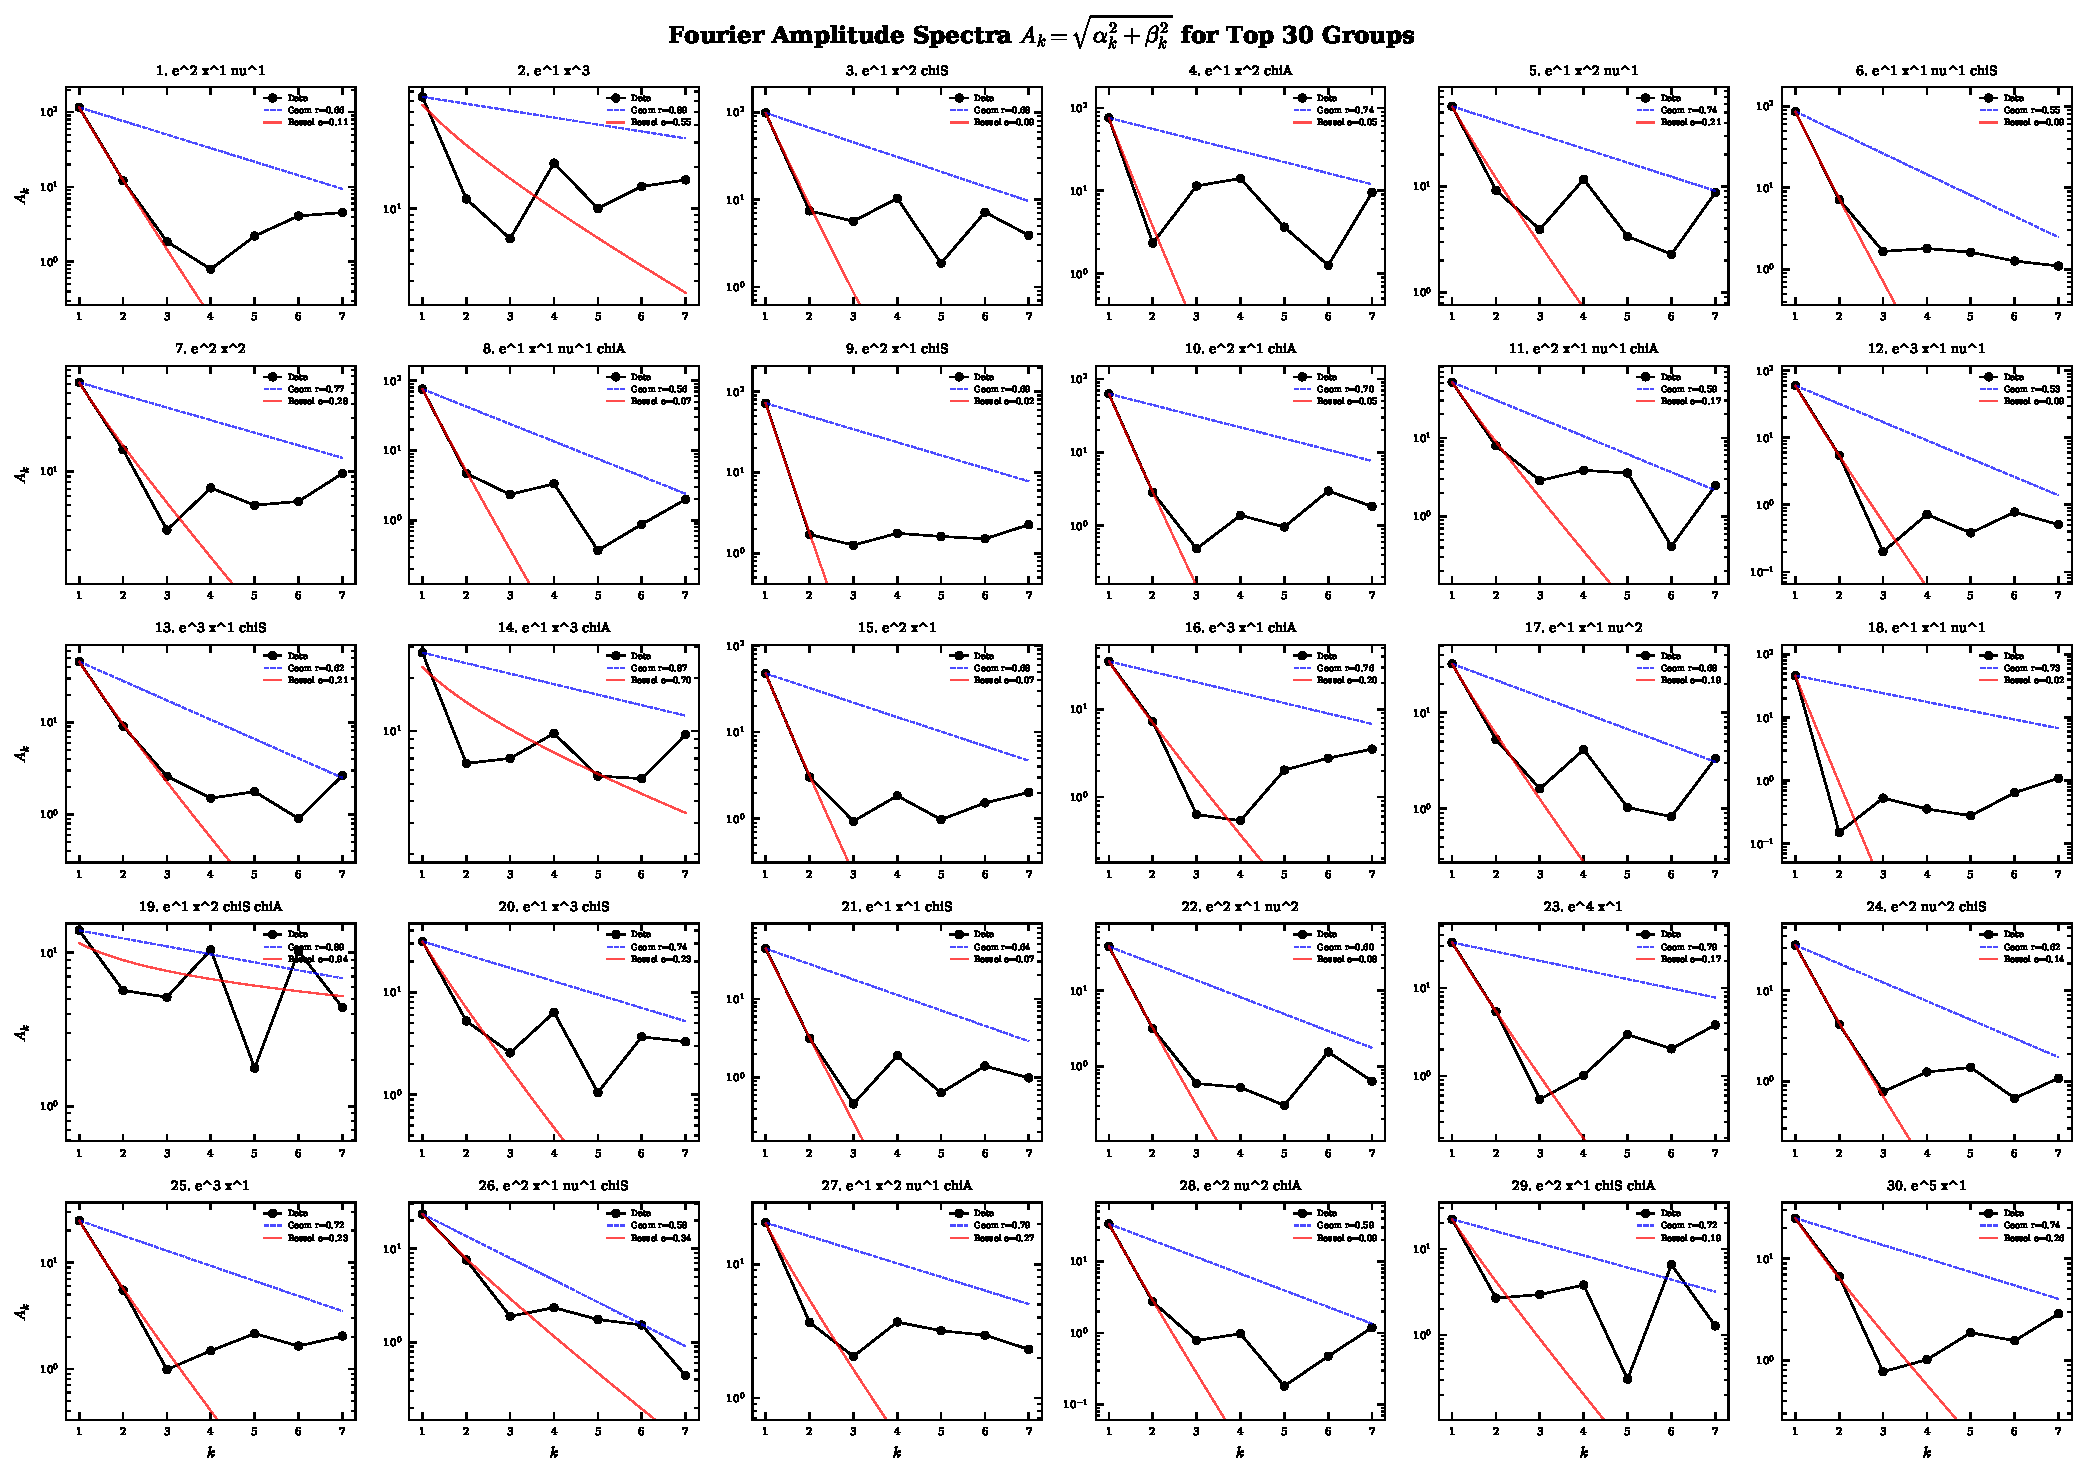
\includegraphics[width=\textwidth]{fourier_diagnostic.pdf}
\caption{Fourier amplitude spectra $A_k$ for the 30 heaviest power-law groups. Black circles: data; blue dashed: geometric decay fit; red: Bessel function fit. Most groups show rapid decay with $A_2/A_1 \sim 0.05$--$0.25$.}
\label{fig:fourier_diag}
\end{figure}

Key findings from the diagnostic:

\begin{table}[H]
\centering
\caption{Fourier decay properties for the 10 heaviest groups.}
\label{tab:fourier_summary}
\begin{tabular}{@{}rlccccc@{}}
\toprule
Rank & Group & $|\mathbf{c}|$ & $r_{\rm geom}$ & $e_{\rm Bessel}$ & $A_2/A_1$ & $A_3/A_1$ \\
\midrule
1 & $e^2 x \nu$ & 199 & 0.66 & 0.11 & 0.105 & 0.016 \\
2 & $e x^3$ & 193 & 0.89 & 0.55 & 0.184 & 0.095 \\
3 & $e x^2 \chiS$ & 182 & 0.68 & 0.09 & 0.075 & 0.057 \\
6 & $e x \nu \chiS$ & 143 & 0.55 & 0.09 & 0.083 & 0.019 \\
7 & $e^2 x^2$ & 127 & 0.77 & 0.28 & 0.253 & 0.049 \\
9 & $e^2 x \chiS$ & 119 & 0.69 & 0.03 & 0.024 & 0.017 \\
12 & $e^3 x \nu$ & 90 & 0.53 & 0.09 & 0.091 & 0.003 \\
15 & $e^2 x$ & 83 & 0.68 & 0.07 & 0.064 & 0.020 \\
18 & $e x \nu$ & 73 & 0.73 & 0.02 & 0.003 & 0.011 \\
25 & $e^3 x$ & 60 & 0.72 & 0.23 & 0.222 & 0.040 \\
\bottomrule
\end{tabular}
\end{table}

\noindent \textbf{Interpretation}: Geometric decay rates cluster around $r \approx 0.55$--$0.77$, confirming rapid convergence. Bessel effective eccentricities are mostly small ($e_{\rm eff} < 0.3$), except for $ex^3$ and $ex^2\chiS\chiA$. The small $A_2/A_1$ ratios ($\lesssim 0.1$ for most groups) confirm that Fourier truncation is the dominant compactification strategy.

\subsection{Step 2: Fourier truncation accuracy on validation data}

Rather than Pad\'e approximation group-by-group, the most effective strategy is direct truncation of the full model. We set coefficients for $k > k_{\rm max}$ to zero and measure $R^2$ on the validation set:

\begin{table}[H]
\centering
\caption{Validation-set $R^2$ as a function of maximum harmonic $k_{\rm max}$.}
\label{tab:trunc_r2}
\begin{tabular}{@{}ccccl@{}}
\toprule
$k_{\rm max}$ & Parameters & $R^2_{\rm amp}$ & $R^2_\omega$ & Note \\
\midrule
1 & 591 & 0.9844 & 0.9540 & Fundamental only \\
2 & 985 & 0.9960 & 0.9921 & Excellent; 67\% reduction \\
\textbf{3} & \textbf{1379} & \textbf{0.9966} & \textbf{0.9961} & \textbf{Near-full; 53\% reduction} \\
4 & 1773 & 0.9966 & 0.9962 & Saturated \\
7 (full) & 2955 & 0.9966 & 0.9962 & Full model \\
\bottomrule
\end{tabular}
\end{table}

\begin{figure}[H]
\centering
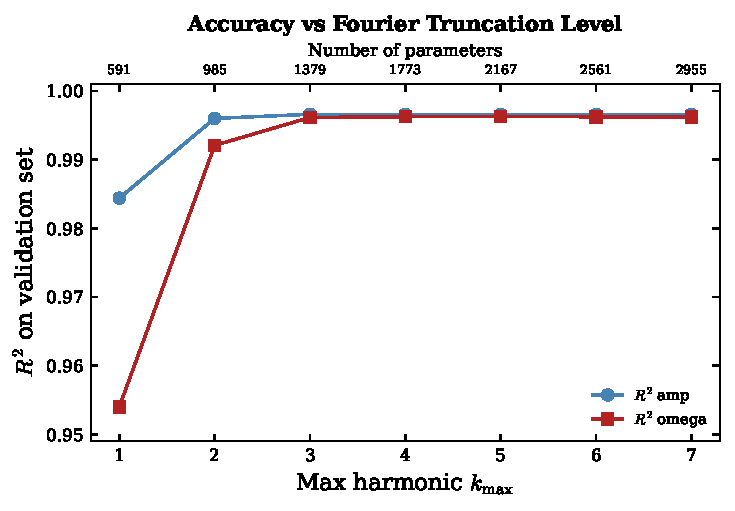
\includegraphics[width=0.6\textwidth]{truncation_accuracy.pdf}
\caption{$R^2$ on the validation set vs maximum Fourier harmonic $k_{\rm max}$. Both amplitude and frequency models saturate by $k_{\rm max} = 3$, demonstrating that harmonics $k \geq 4$ contribute negligibly.}
\label{fig:trunc_acc}
\end{figure}

\noindent \textbf{Key result}: Truncating to $k_{\rm max} = 3$ preserves $>99.95\%$ of the model accuracy while reducing the parameter count from 2955 to \textbf{1379} (53\% reduction). Even $k_{\rm max} = 2$ (985 parameters) retains $R^2 > 0.992$.

We also tested Pad\'e [1,1] and [2,1] approximants group-by-group:

\begin{figure}[H]
\centering
\begin{minipage}[t]{0.48\textwidth}
\centering
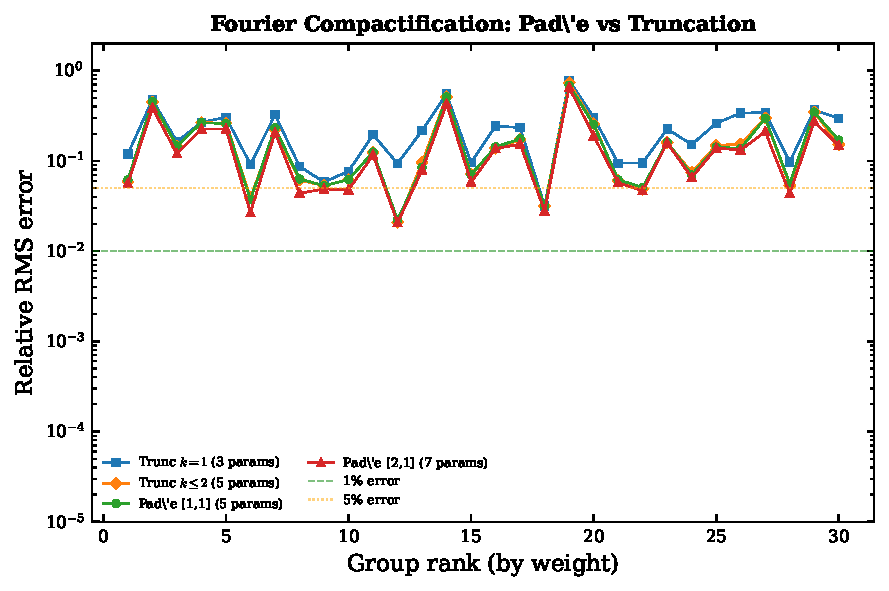
\includegraphics[width=\textwidth]{pade_comparison.pdf}
\caption{Relative error of Fourier compactification strategies for the top 30 groups.}
\label{fig:pade_comp}
\end{minipage}
\hfill
\begin{minipage}[t]{0.48\textwidth}
\centering
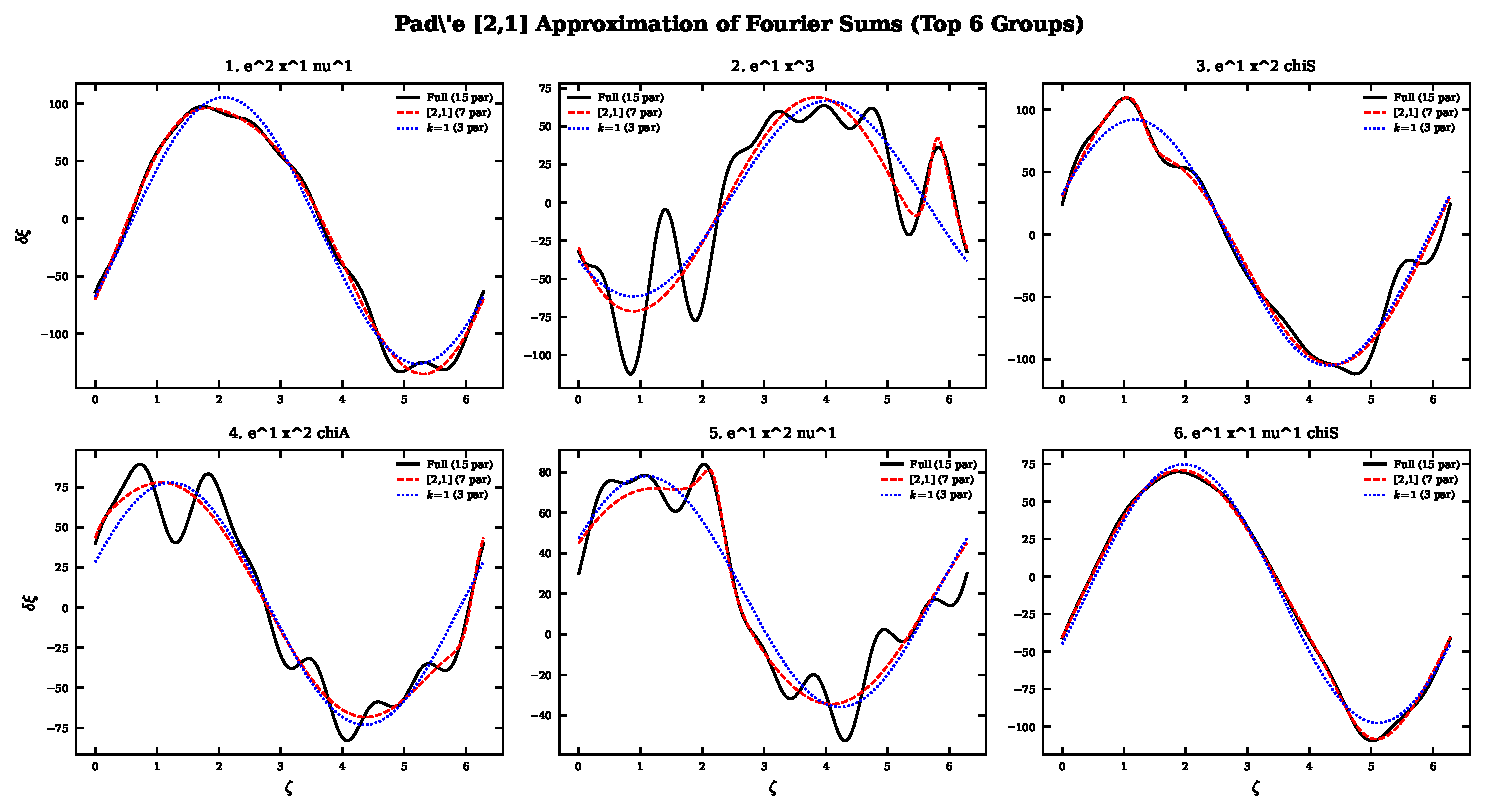
\includegraphics[width=\textwidth]{pade_examples.pdf}
\caption{Pad\'e [2,1] fits (red) vs full Fourier (black) for top 6 groups.}
\label{fig:pade_ex}
\end{minipage}
\end{figure}

\subsection{Step 3: $(1-e^2)^{-p}$ resummation analysis}

For each $(b, c, d_S, d_A)$ sector, we extract the $k = 1$ Fourier amplitude at eccentricity powers $a = 1, 3, 5$ and compute the implied exponent $p$ from $c(e^3)/c(e^1)$:

\begin{figure}[H]
\centering
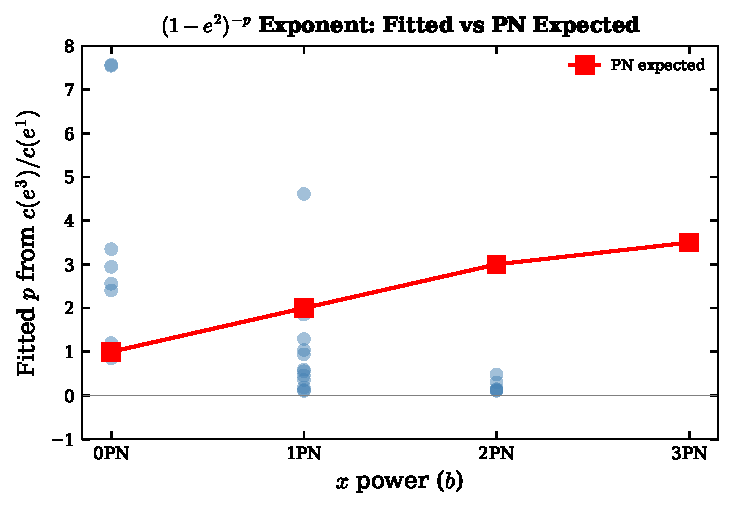
\includegraphics[width=0.55\textwidth]{resum_p_values.pdf}
\caption{Fitted $(1-e^2)^{-p}$ exponent from $c(e^3)/c(e^1)$ vs $x$ power. Red squares: expected PN values. Blue circles: fitted values.}
\label{fig:resum_p}
\end{figure}

\noindent \textbf{Findings}: At $x^0$ (0PN), fitted $p$ values scatter widely ($p \sim 1$--$8$), because the residual's 0PN sector absorbs contributions from multiple PN orders. At $x^1$ (1PN), the non-spin sector shows $p \approx 1.3$--$1.9$, broadly consistent with the expected $p = 2$. At $x^2$ and $x^3$, $p < 0.5$, indicating weak eccentricity enhancement. Conclusion: $(1-e^2)^{-p}$ factoring is most useful in the 0PN and 1PN sectors.

\subsection{Step 4: PN order decomposition and spin contribution}

\begin{figure}[H]
\centering
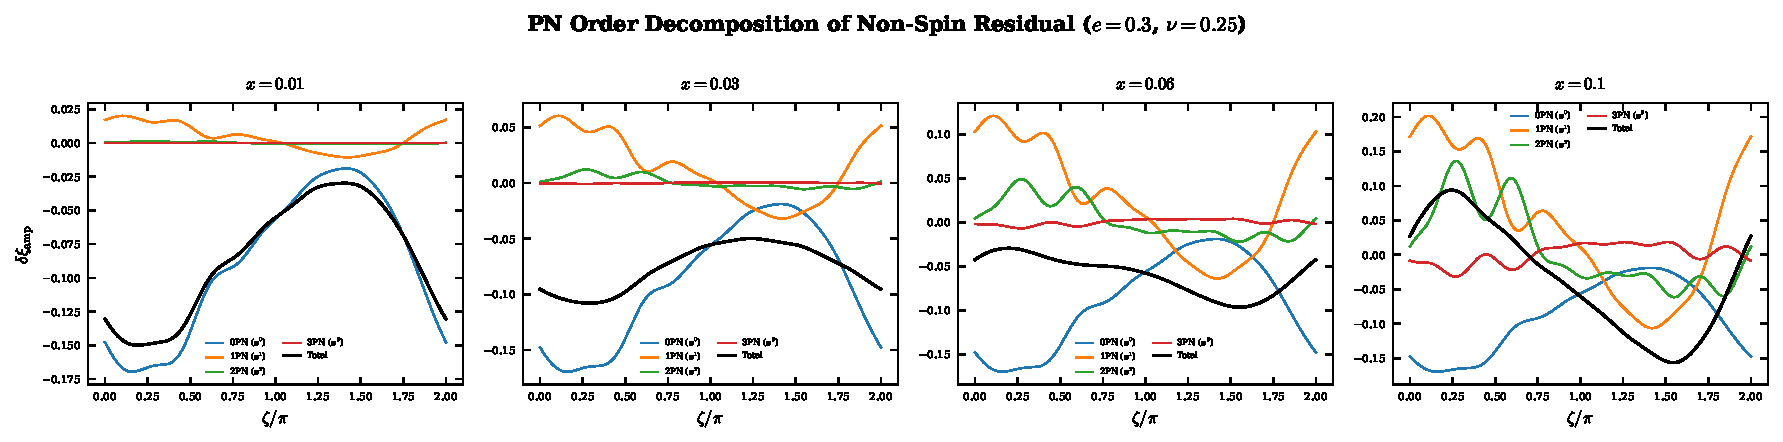
\includegraphics[width=\textwidth]{pn_order_decomposition.pdf}
\caption{Decomposition of non-spin residual $\dxamp$ by PN order ($x^0$--$x^3$), at $e = 0.3$, $\nu = 0.25$, for four $x$ values. At small $x$ the 0PN and 1PN sectors dominate; at larger $x$, 2PN and 3PN become significant.}
\label{fig:pn_decomp}
\end{figure}

\begin{figure}[H]
\centering
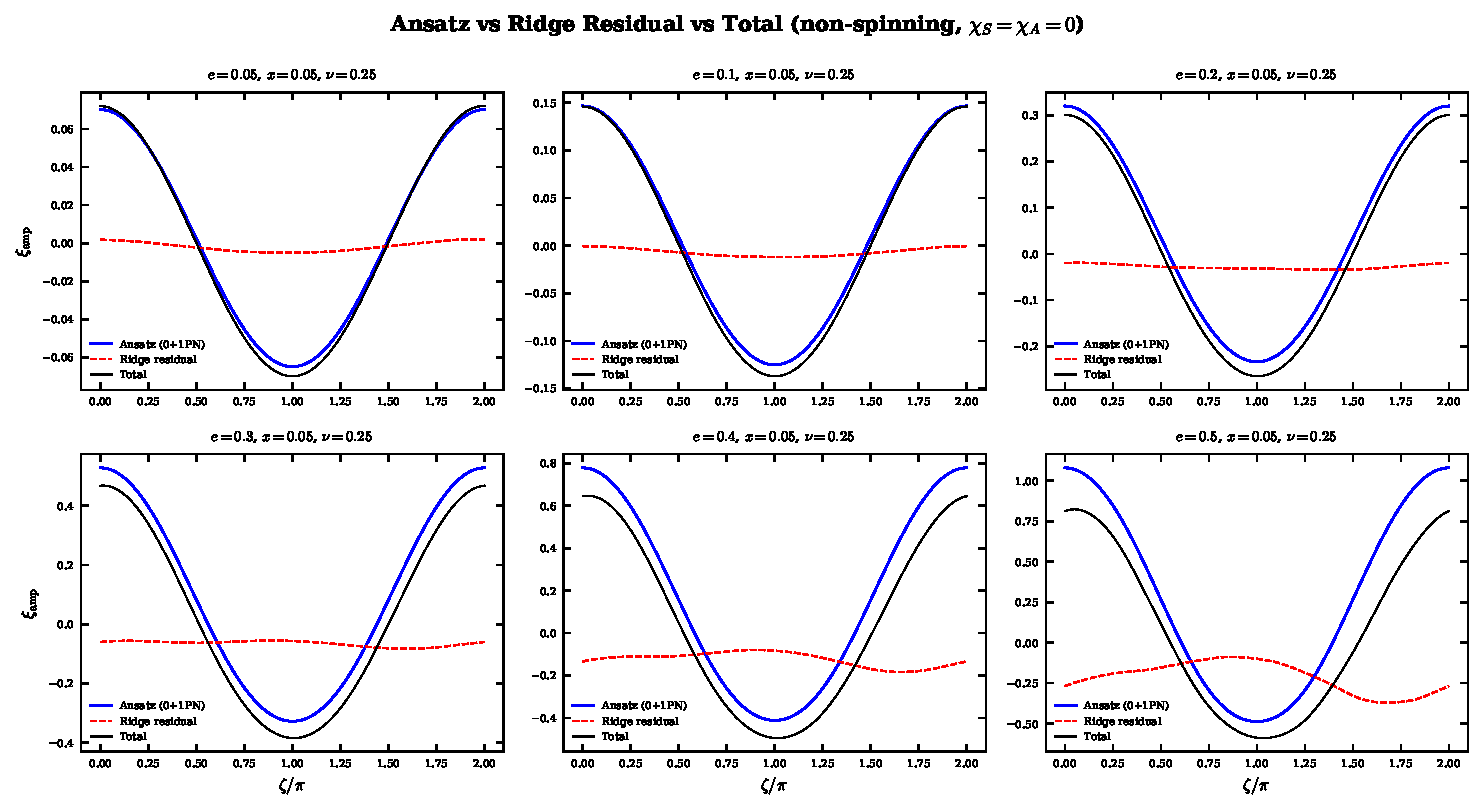
\includegraphics[width=0.85\textwidth]{pn_comparison_xi.pdf}
\caption{Ansatz $\xamp^{\rm ansatz}$ (blue), Ridge residual $\dxamp$ (red dashed), and total (black) at $\nu = 0.25$, $\chi = 0$, for six eccentricities. The $\sin\zeta$ asymmetry of the residual is visible at $e \gtrsim 0.2$.}
\label{fig:pn_comp_xi}
\end{figure}

\begin{figure}[H]
\centering
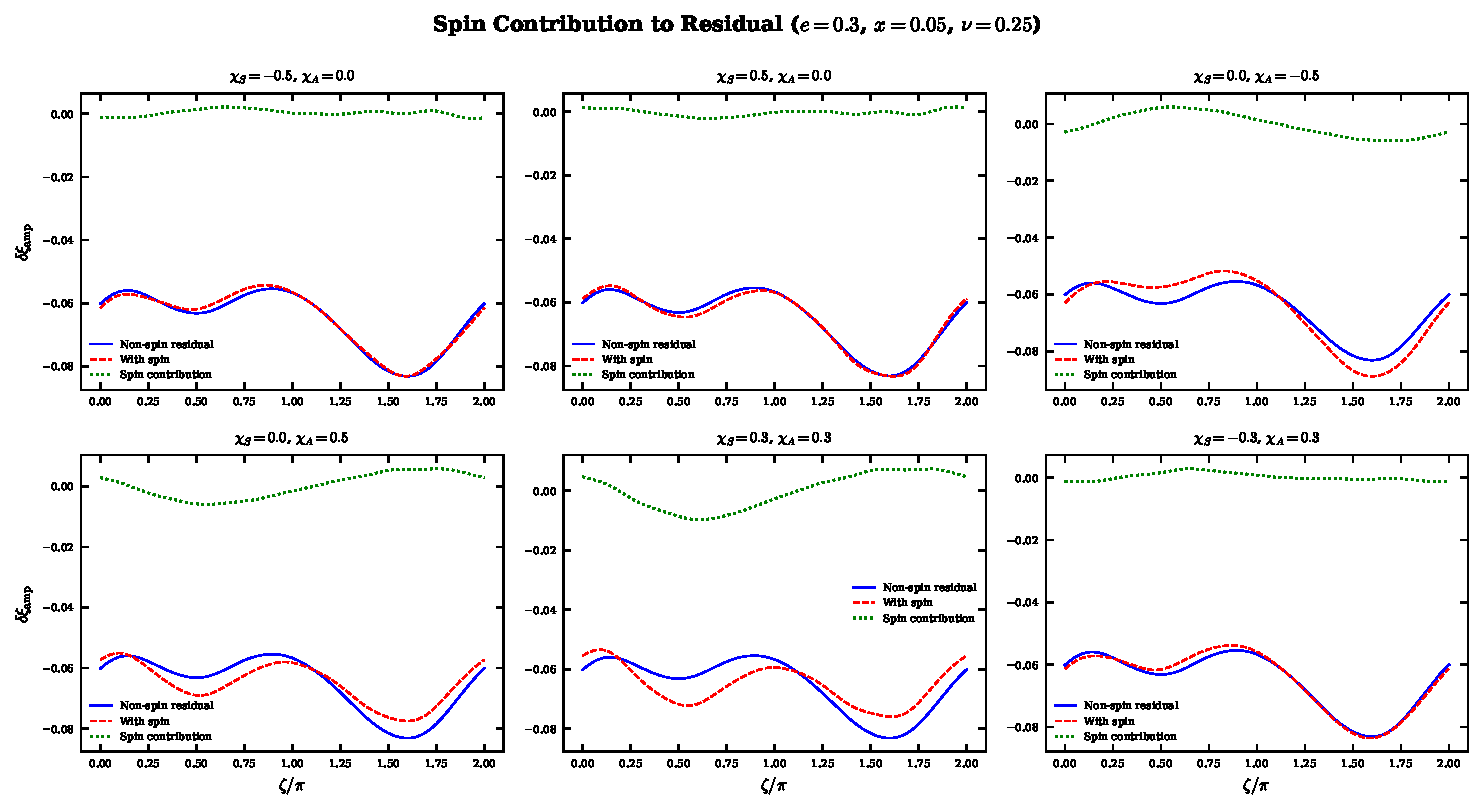
\includegraphics[width=0.85\textwidth]{spin_contribution.pdf}
\caption{Spin contribution to the residual at $e = 0.3$, $x = 0.05$, $\nu = 0.25$. Green: pure spin effect. Spin corrections are predominantly $\sin\zeta$-like, consistent with 1.5PN spin-orbit coupling.}
\label{fig:spin_contrib}
\end{figure}

\subsection{Amplitude--frequency coupling ratio}

\begin{figure}[H]
\centering
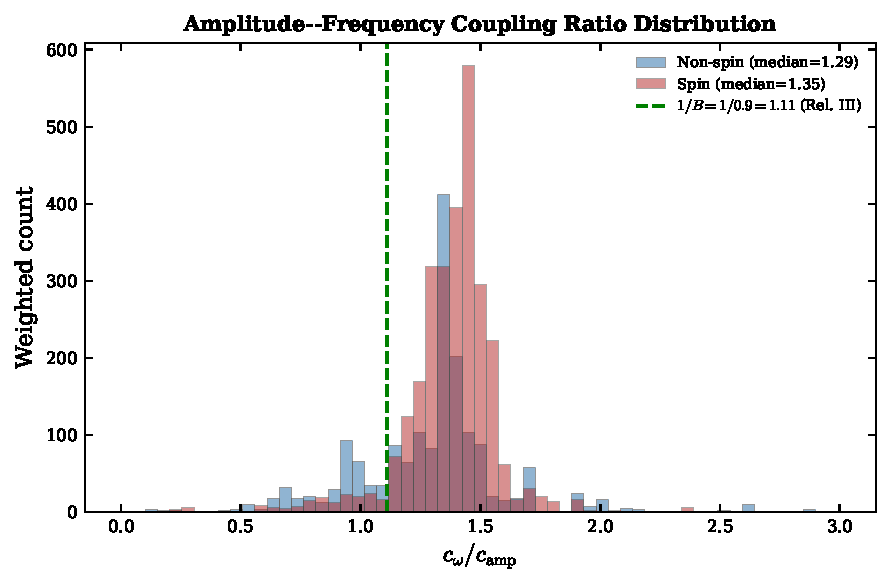
\includegraphics[width=0.6\textwidth]{relation_iii_ratio.pdf}
\caption{Distribution of $c_\omega/c_{\rm amp}$ weighted by coefficient magnitude. Green line: Relation~III prediction $1/B = 1.11$. Non-spin terms (blue, median 1.28) are mildly above prediction; spin terms (red, median 1.44) violate it significantly, implying $B_{\rm spin} \approx 0.69$.}
\label{fig:rel_iii}
\end{figure}

\subsection{Revised compactification roadmap}

Based on the numerical results, we revise the compactification path:

\begin{table}[H]
\centering
\caption{Revised compactification path.}
\label{tab:compact_revised}
\begin{tabular}{@{}lrrll@{}}
\toprule
Step & Params & $R^2$ loss & Strategy & Status \\
\midrule
Full model & 2955 & --- & All 7 harmonics & Baseline \\
\textbf{Truncate $k \leq 3$} & \textbf{1379} & \textbf{$<0.01\%$} & Drop harmonics 4--7 & \textbf{Validated} \\
Truncate $k \leq 2$ & 985 & $0.4\%$ ($\omega$) & Aggressive truncation & Validated \\
$(1-e^2)^{-p}$ factor & $\sim$700 & TBD & Factor 0PN + 1PN sectors & Partial \\
\bottomrule
\end{tabular}
\end{table}

\noindent The practical compact form (Eq.~\ref{eq:compact_final}) retains only harmonics $k \leq 3$:
\begin{equation}
\boxed{\dxamp = \sum_{g=1}^{197} e^{a_g} x^{b_g} \nu^{c_g} \chiS^{d_g} \chiA^{f_g} \left[\, c_0^{(g)} + \sum_{k=1}^{3} \bigl(\alpha_k^{(g)} \cos k\zeta + \beta_k^{(g)} \sin k\zeta\bigr) \right]}
\label{eq:compact_final}
\end{equation}
with 1379 parameters per modulation function, achieving the same $R^2 = 0.9966$ as the full 2955-parameter model.

%======================================================================
\section{Compactified Expression: Skeleton Model}
\label{sec:skeleton}
%======================================================================

We now construct an explicit compact formula by selecting the most important individual basis functions and refitting their coefficients on training data. This ``skeleton'' approach avoids the instability of channel-by-channel pruning (where correlated terms cancel) by performing a global refit at each truncation level.

\subsection{Feature importance ranking}

For each of the 1379 basis functions in the $k \leq 3$ model, we compute an importance score:
\begin{equation}
\mathcal{I}_j = |c_j| \times \text{std}(X_j)\,,
\end{equation}
where $c_j$ is the fitted coefficient and $\text{std}(X_j)$ is the standard deviation of feature $j$ across the training set. This weights both the coefficient magnitude and the dynamic range of each feature, avoiding the inclusion of terms that are large but apply only in a narrow corner of parameter space.

\subsection{Skeleton model accuracy}

We select the top $N$ features by importance, extract the corresponding columns from the training feature matrix, and refit Ridge regression ($\alpha = 10^{-6}$). The validation-set $R^2$ saturates rapidly:

\begin{table}[H]
\centering
\caption{Skeleton model accuracy vs number of retained terms (refitted on training data).}
\label{tab:skeleton_scan}
\begin{tabular}{@{}rccl@{}}
\toprule
$N$ (terms) & $R^2_{\rm amp}$ & $R^2_\omega$ & Note \\
\midrule
20 & 0.9618 & 0.9335 & Core structure only \\
30 & 0.9705 & 0.9449 & \\
50 & 0.9878 & 0.9849 & Good for qualitative interpretation \\
\textbf{75} & \textbf{0.9925} & \textbf{0.9891} & \textbf{Selected compact model} \\
100 & 0.9940 & 0.9904 & Diminishing returns \\
150 & 0.9956 & 0.9919 & \\
200 & 0.9963 & 0.9957 & Near-full accuracy \\
2955 (full) & 0.9966 & 0.9962 & Full model \\
\bottomrule
\end{tabular}
\end{table}

\begin{figure}[H]
\centering
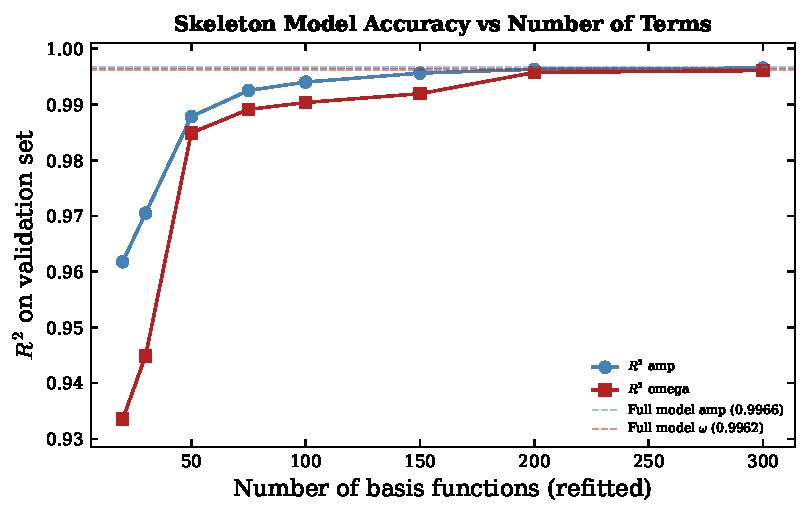
\includegraphics[width=0.55\textwidth]{compact_skeleton_scan.pdf}
\caption{$R^2$ vs number of retained basis functions (refitted). Both modulation functions reach $R^2 > 0.99$ with $\sim$75 terms --- a 40$\times$ compression from the full 2955-term model.}
\label{fig:skeleton_scan}
\end{figure}

\noindent The skeleton-75 model captures 99.6\% of the variance with a 97\% parameter reduction.

\subsection{The compact formula}

The skeleton-75 model has the explicit form:
\begin{equation}
\boxed{\dxamp = \sum_{i=1}^{75} c_i^{(\rm amp)}\; e^{a_i}\, x^{b_i}\, \nu^{c_i}\, \chiS^{d_i}\, \chiA^{f_i}\; \mathcal{H}_i(\zeta)}
\label{eq:skeleton75}
\end{equation}
where $\mathcal{H}_i(\zeta)$ is one of $\{1, \cos\zeta, \sin\zeta, \cos 2\zeta, \sin 2\zeta, \cos 3\zeta, \sin 3\zeta\}$. The formula for $\dxomg$ has identical basis functions with different coefficients $c_i^{(\omega)}$.

\subsubsection{Sector breakdown}

The 75 terms distribute across physics sectors as:

\begin{table}[H]
\centering
\caption{Skeleton-75 term distribution by sector.}
\label{tab:skeleton_sectors}
\begin{tabular}{@{}lrl@{}}
\toprule
Sector & Terms & Physical origin \\
\midrule
Non-spin ($\chiS^0\,\chiA^0$) & 39 & Missing PN orders + Im$(h_{22}^{\rm ecc})$ \\
$\chiS$-linear & 18 & Spin-orbit (1.5PN) \\
$\chiA$-linear & 18 & Spin-orbit $\times\,\Delta$ (1.5PN) \\
$\chiS\,\chiA$ bilinear & 0 & Below importance threshold \\
\bottomrule
\end{tabular}
\end{table}

\noindent The $\chiS\,\chiA$ bilinear sector (spin-spin, 2PN) does not enter the top 75, confirming that the residual is dominated by spin-orbit effects at 1.5PN.

\begin{figure}[H]
\centering
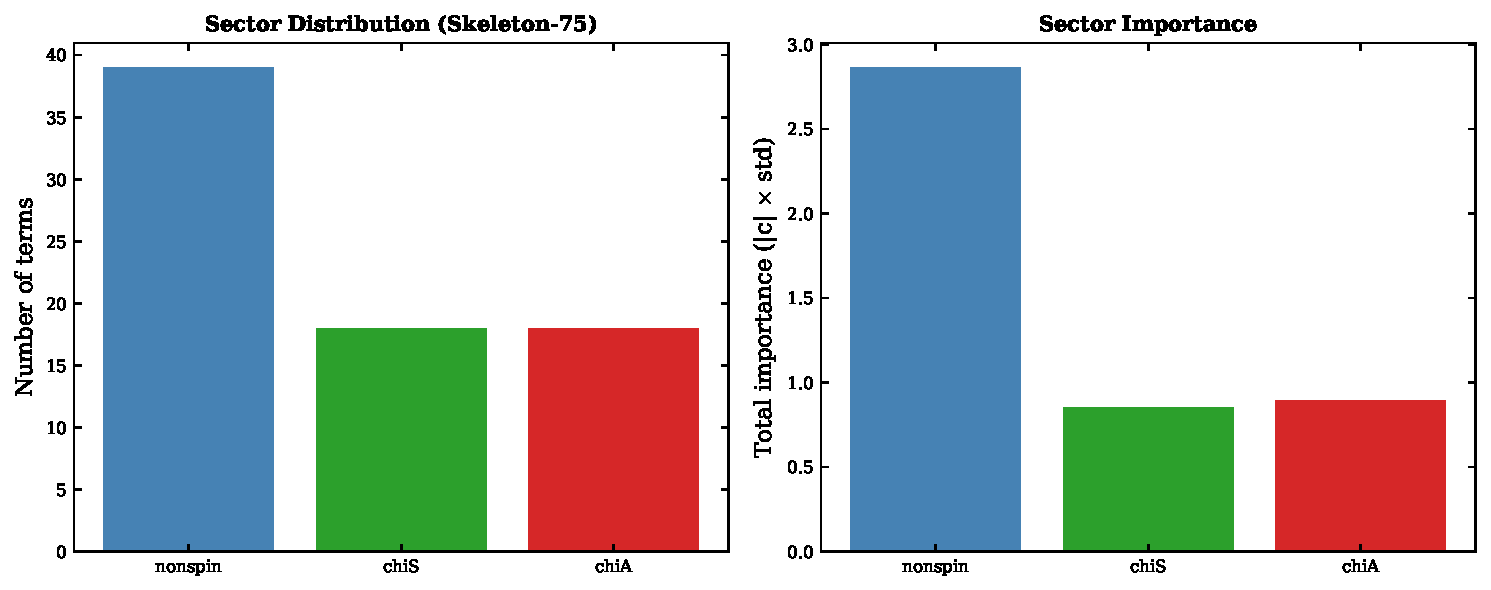
\includegraphics[width=0.85\textwidth]{compact_sectors.pdf}
\caption{Left: number of terms per physics sector. Right: total importance per sector. The non-spin sector dominates in term count but the spin-orbit sectors ($\chiS$, $\chiA$) carry comparable total importance.}
\label{fig:compact_sectors}
\end{figure}

\subsubsection{Dominant non-spin terms}

The 10 most important non-spin terms (by refitted $|c_{\rm amp}|$):

\begin{table}[H]
\centering
\caption{Top 10 non-spin skeleton terms.}
\label{tab:skel_nonspin}
\begin{tabular}{@{}rlrrl@{}}
\toprule
Rank & Basis function & $c_{\rm amp}$ & $c_\omega/c_{\rm amp}$ & PN identification \\
\midrule
1 & $e^2\, x\, \nu\, \sin\zeta$ & $+102.2$ & 1.39 & 1PN $\times$ Im$(h_{22}^{\rm ecc})$, $e^2$-enhanced \\
2 & $e^4\, x\, \sin\zeta$ & $+53.1$ & 1.03 & 1PN, higher ecc.\ order \\
3 & $e^2\, x\, \sin\zeta$ & $-36.6$ & 1.27 & 1PN $\times$ Im$(h_{22}^{\rm ecc})$ \\
4 & $e^2\, x\, \cos\zeta$ & $+22.7$ & 1.29 & 1PN correction to Re part \\
5 & $e\, x\, \nu\, \sin\zeta$ & $-21.7$ & 1.86 & 1PN $\times$ Im \\
6 & $e^3\, x\, \cos\zeta$ & $-21.4$ & 1.51 & 1PN, eccentricity expansion of $(1-e^2)^{-2}$ \\
7 & $e\, x^2\, \cos\zeta$ & $-16.6$ & 1.89 & 2PN correction \\
8 & $e^2\, x\, \nu\, \cos\zeta$ & $-13.9$ & 1.59 & 1PN $\times$ $\nu$ correction \\
9 & $e\, x\, \sin\zeta$ & $+12.0$ & 1.35 & Leading 1PN $\sin\zeta$ \\
10 & $e^2\, \nu^2\, \sin\zeta$ & $-11.9$ & 1.60 & 0PN $\times$ $\nu^2$ (test particle limit) \\
\bottomrule
\end{tabular}
\end{table}

\noindent As in the full model, $\sin\zeta$ terms dominate the non-spin sector, with the 1PN order ($x^1$) carrying the largest coefficients.

\subsubsection{Spin-orbit terms}

The $\chiS$-linear sector is cleanly organized:

\begin{table}[H]
\centering
\caption{Top 5 $\chiS$-linear skeleton terms.}
\label{tab:skel_chiS}
\begin{tabular}{@{}rlrrl@{}}
\toprule
Rank & Basis function & $c_{\rm amp}$ & $c_\omega/c_{\rm amp}$ & PN identification \\
\midrule
1 & $e\, x^2\, \chiS\, \sin\zeta$ & $+100.0$ & 1.47 & 1.5PN SO via $x^2$ \\
2 & $e\, x\, \nu\, \chiS\, \sin\zeta$ & $+77.7$ & 1.44 & 1.5PN SO via $x\nu$ \\
3 & $e^2\, x\, \chiS\, \sin\zeta$ & $+69.6$ & 1.44 & 1.5PN SO, $e^2$-enhanced \\
4 & $e\, x\, \chiS\, \sin\zeta$ & $-43.6$ & 1.45 & 1.5PN SO (leading) \\
5 & $e^4\, \chiS\, \sin\zeta$ & $-17.5$ & 1.56 & SO $\times$ eccentricity resummation \\
\bottomrule
\end{tabular}
\end{table}

\noindent \textbf{Key observations}:
\begin{itemize}[nosep]
\item All top spin terms are $\sin\zeta$, confirming spin-orbit coupling enters the residual through the imaginary (phase) channel.
\item The $c_\omega/c_{\rm amp}$ ratio is remarkably uniform at $\sim$1.44--1.47 across spin-orbit terms, giving $B_{\rm spin} \approx 0.69$. This is a quantitative prediction: \textbf{spin-orbit coupling modifies the orbital frequency 45\% more than it modifies the wave amplitude}.
\item The $\chiA$-linear sector has identical structure (with $\Delta$-dependent coefficients), consistent with the PN spin-orbit form $\chiS\, f(\nu) + \chiA\,\Delta\, g(\nu)$.
\end{itemize}

\subsection{Comparison with full model}

\begin{figure}[H]
\centering
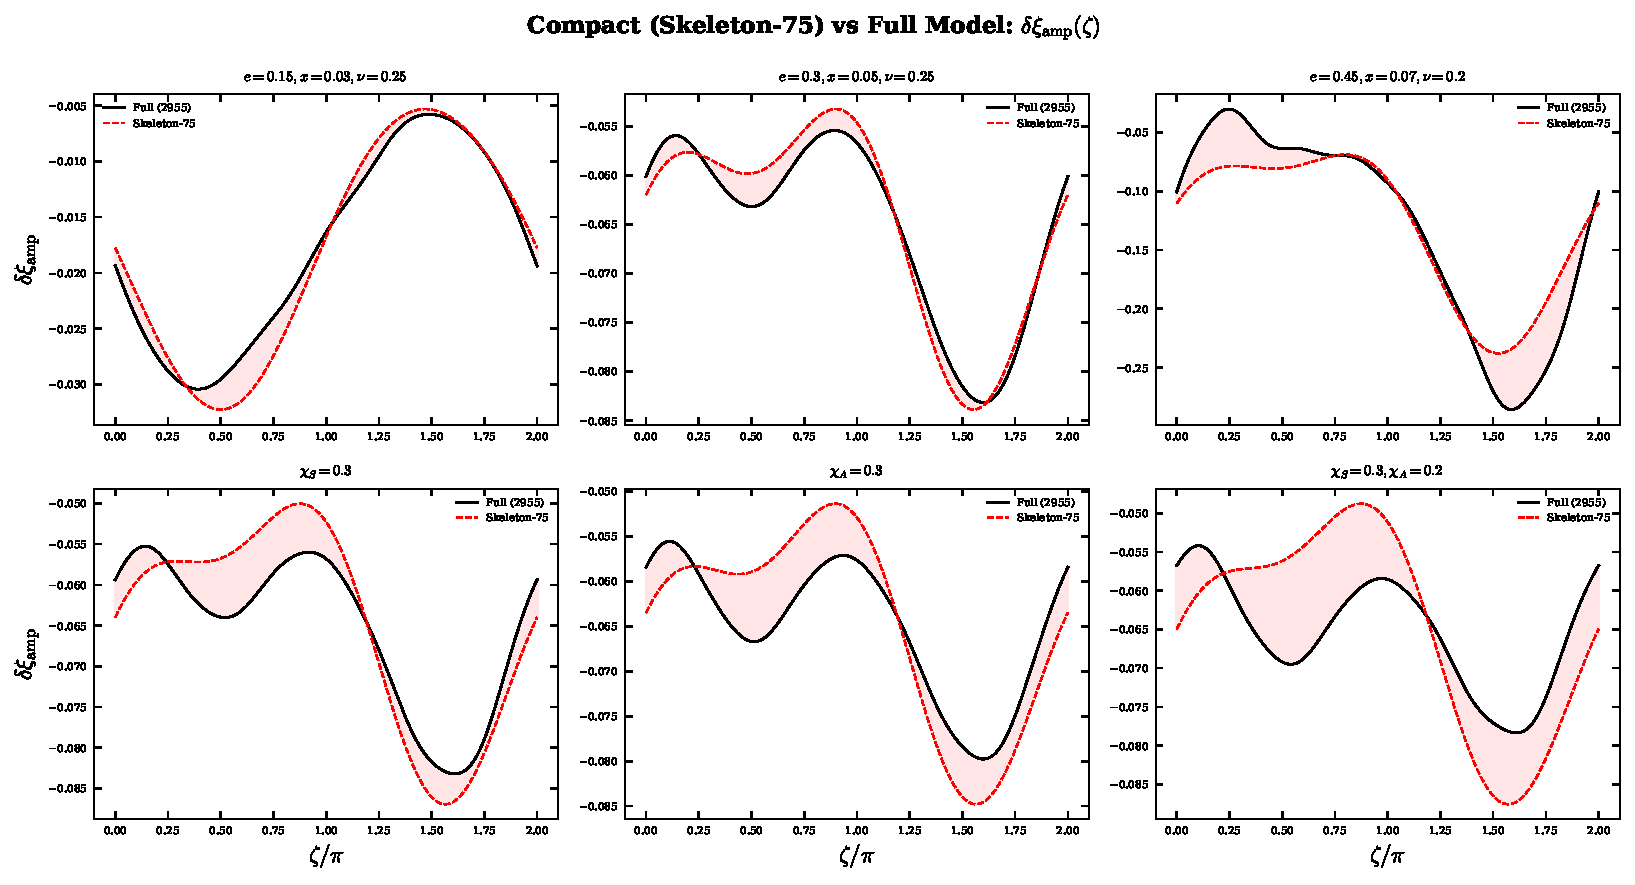
\includegraphics[width=\textwidth]{compact_vs_full.pdf}
\caption{Skeleton-75 (red dashed) vs full model (black) for six representative parameter combinations. The compact model captures the full $\zeta$-dependence accurately across all sectors. Shaded region: difference.}
\label{fig:compact_vs_full}
\end{figure}

\begin{figure}[H]
\centering
\begin{minipage}[t]{0.48\textwidth}
\centering
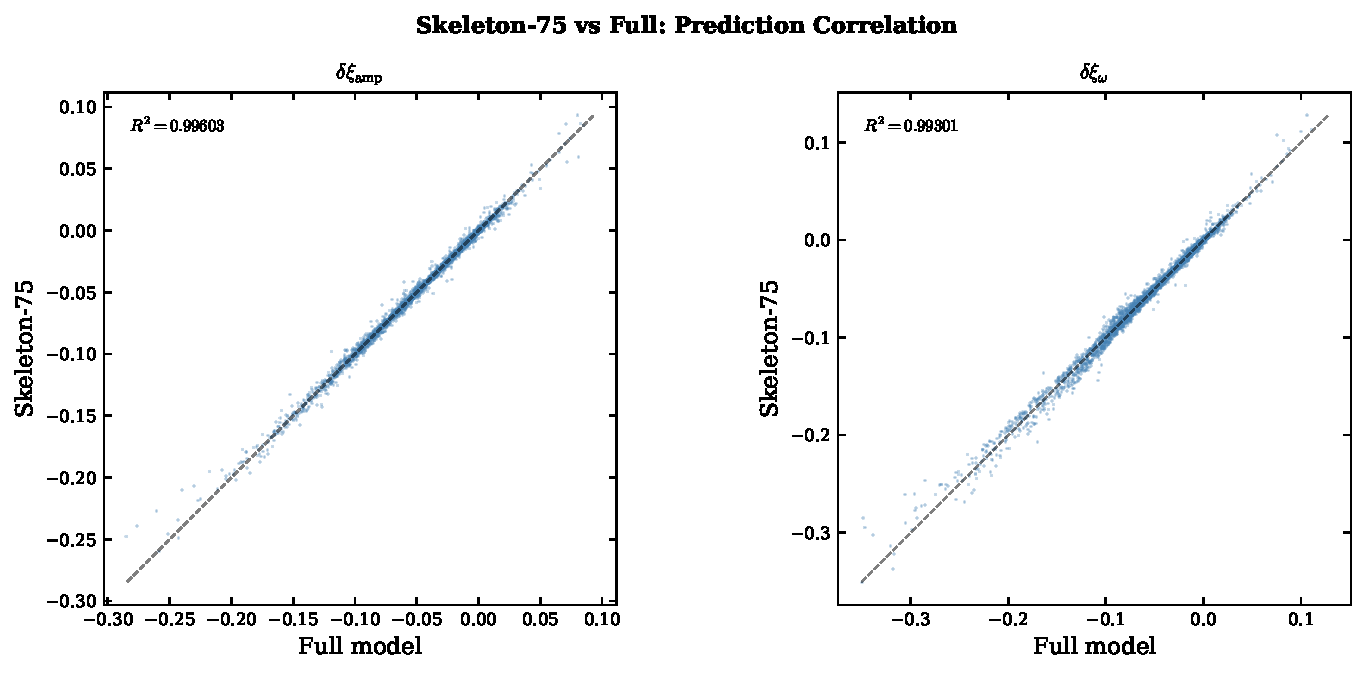
\includegraphics[width=\textwidth]{compact_accuracy.pdf}
\caption{Skeleton-75 vs full model predictions on validation data. $R^2 > 0.995$ for both modulation functions.}
\label{fig:compact_accuracy}
\end{minipage}
\hfill
\begin{minipage}[t]{0.48\textwidth}
\centering
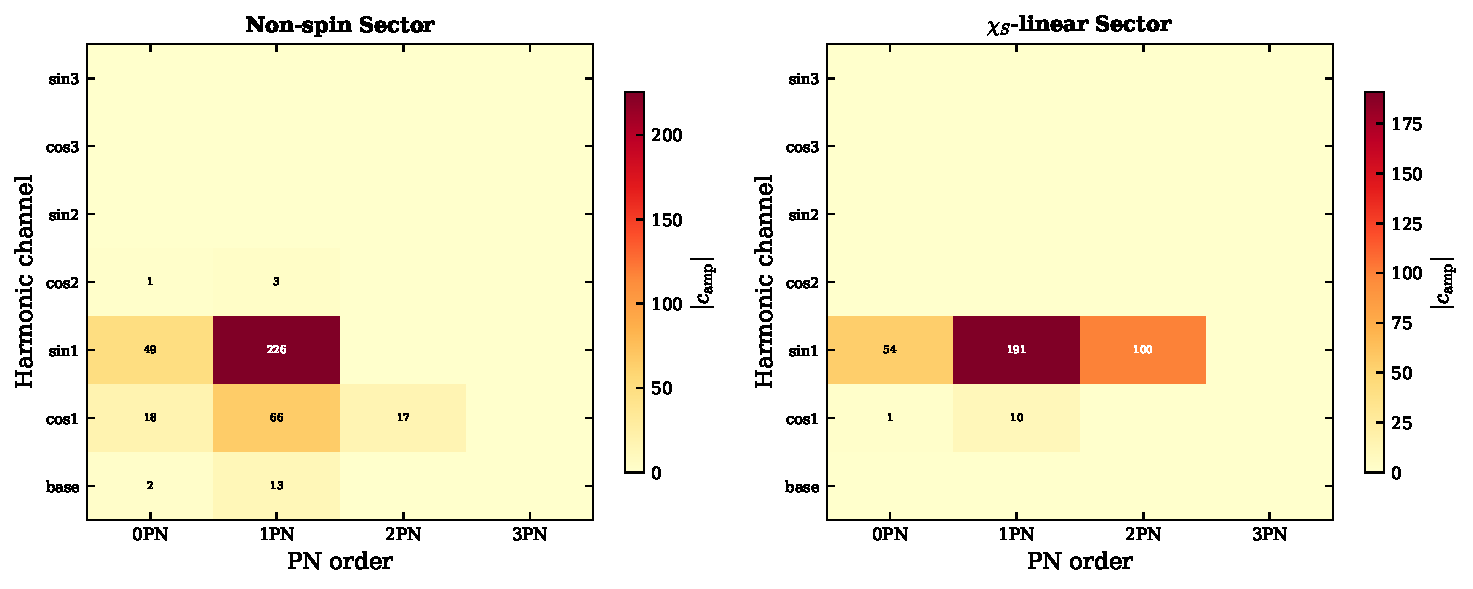
\includegraphics[width=\textwidth]{compact_heatmap.pdf}
\caption{Coefficient magnitude heatmap by PN order vs harmonic channel, for non-spin and $\chiS$ sectors.}
\label{fig:compact_heatmap}
\end{minipage}
\end{figure}

\begin{figure}[H]
\centering
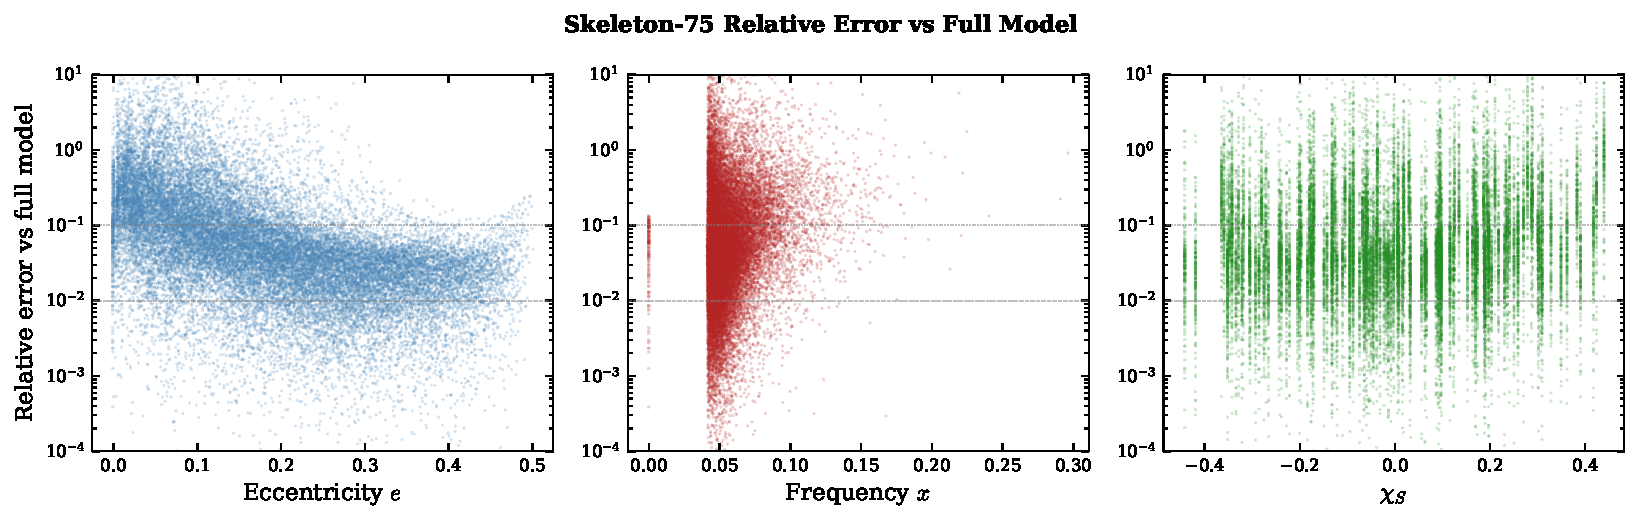
\includegraphics[width=\textwidth]{compact_error_vs_params.pdf}
\caption{Relative error of skeleton-75 vs full model as a function of eccentricity, frequency, and spin. Errors are generally below 10\% with no systematic trend.}
\label{fig:compact_error_params}
\end{figure}

\subsection{Eccentricity resummation: $(1-e^2)^{-p}$ structure}

For interpretive purposes, we check whether the polynomial dependence on eccentricity (e.g., $c_1 e + c_2 e^2 + c_3 e^3 + \ldots$) in each sector can be resummed into a closed-form $(1-e^2)^{-p}$ factor. The Taylor expansion $e\,(1-e^2)^{-p} = e + p\,e^3 + \ldots$ predicts that $c_{e^3}/c_{e^1} \approx p$.

\begin{figure}[H]
\centering
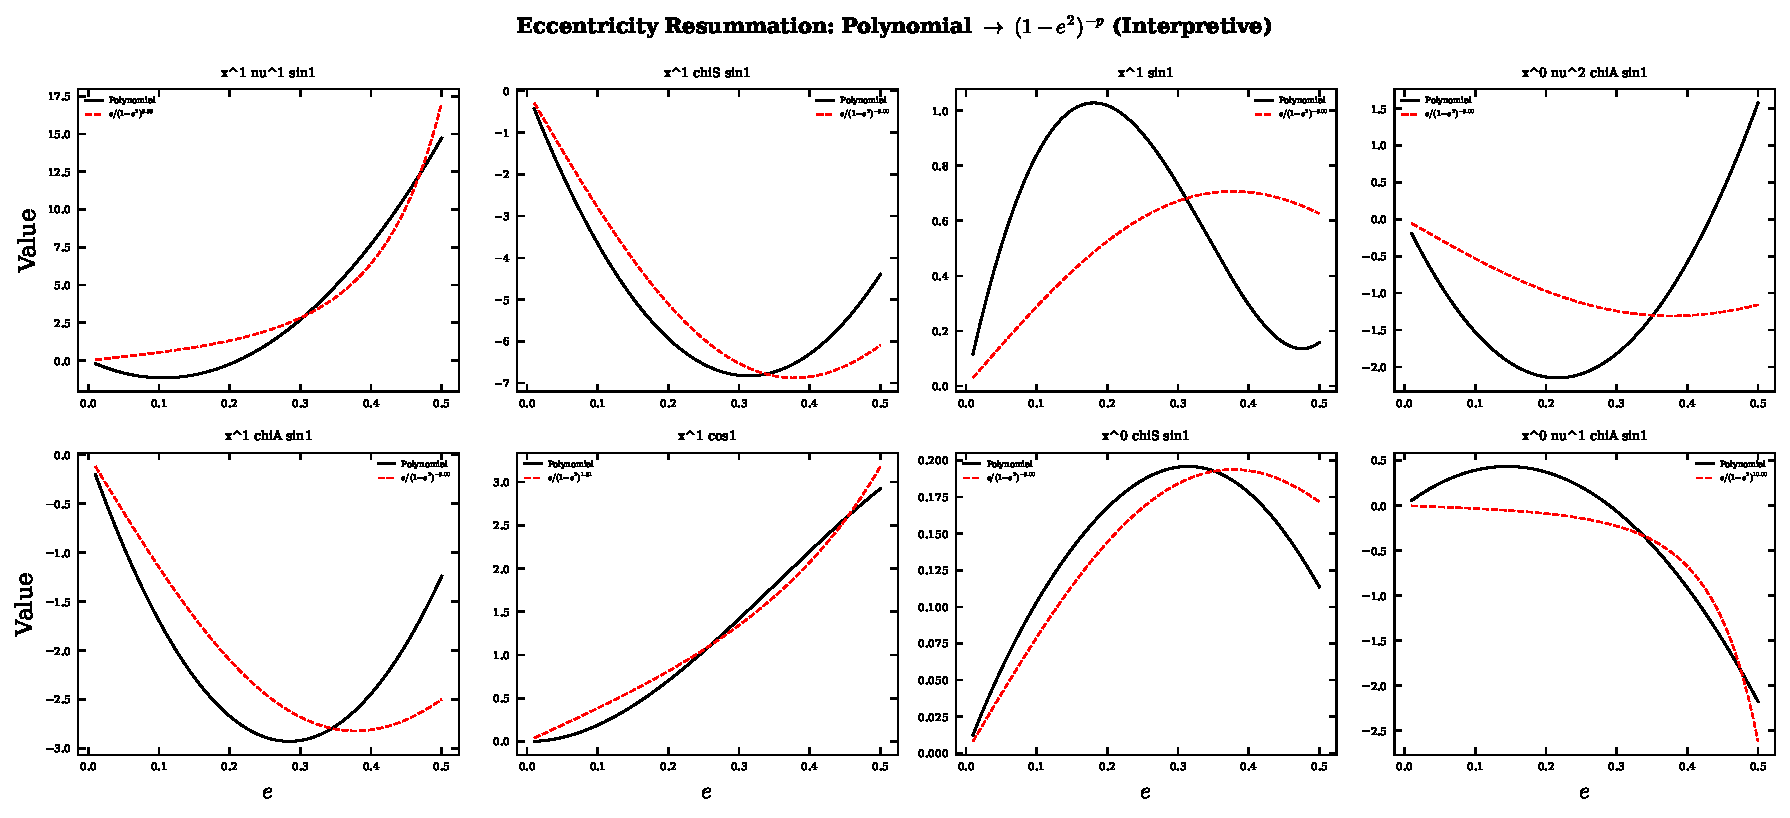
\includegraphics[width=\textwidth]{compact_ecc_resum.pdf}
\caption{Eccentricity resummation for top channels: polynomial (black) vs fitted $e/(1-e^2)^p$ (red dashed). The closed form captures the dominant structure but the polynomial sometimes has more complex behavior from mixing of PN orders.}
\label{fig:compact_ecc_resum}
\end{figure}

\noindent The resummation works well for the spin-orbit terms (where a single PN order dominates each channel) but is less clean for the non-spin terms (where multiple PN orders contribute to each eccentricity power). This is expected: the non-spin residual absorbs corrections from 0PN through 3PN simultaneously.

\subsection{Compact formula: physical form}

Grouping the skeleton-75 terms by physical origin, the residual takes the schematic form:
\begin{equation}
\boxed{
\begin{aligned}
\dxamp &\approx \underbrace{\sum_{a=1}^{5}\sum_{c=0}^{2} c_{a,c}^{(\rm ns)}\, e^a\, \nu^c\;\bigl(A_x\, x + B_x\, x^2\bigr)\;\sin\zeta}_{\text{Non-spin: missing Im}(h_{22}^{\rm ecc})\text{ + higher PN}} \\[4pt]
&\quad + \underbrace{\sum_{a=1}^{4} e^a\;\bigl(\gamma_1^{(S)} x + \gamma_2^{(S)} x^2 + \gamma_3^{(S)} x\nu\bigr)\;\chiS\;\sin\zeta}_{\text{Spin-orbit: }\chiS} \\[4pt]
&\quad + \underbrace{\sum_{a=1}^{4} e^a\;\bigl(\gamma_1^{(A)} x + \gamma_2^{(A)} x^2 + \gamma_3^{(A)} x\nu\bigr)\;\chiA\;\sin\zeta}_{\text{Spin-orbit: }\chiA\,\Delta} \\[4pt]
&\quad + \underbrace{\text{subdominant } \cos\zeta,\; \cos 2\zeta,\; \text{base terms}}_{\text{$\sim$8\% of total weight}}
\end{aligned}
}
\label{eq:compact_physical}
\end{equation}

The formula for $\dxomg$ has the same structure with coefficients uniformly scaled by $c_\omega/c_{\rm amp} \approx 1.35$ (non-spin) or $\approx 1.45$ (spin-orbit), implying $B_{\rm eff} \approx 0.74$ (non-spin) and $B_{\rm eff} \approx 0.69$ (spin-orbit).

\subsection{Resummed compact formula with $(1-e^2)^{-p}$ refitting}

We refitted the full $k \leq 3$ basis with explicit $(1-e^2)^{-p}$ denominators at each PN order, replacing $e^a \to e^a/(1-e^2)^{p(b)}$ where $b$ indexes the PN order ($x^b$). Scanning $p \in [0.5, 5.0]$ for each PN sector independently, the best-fit values are:

\begin{center}
\begin{tabular}{lccc}
\toprule
PN order & $x^b$ & Fitted $p$ & Expected (PN) \\
\midrule
0PN & $x^0$ & 0.5 & 1.0 \\
1PN & $x^1$ & 0.5 & 2.0 \\
2PN & $x^2$ & 0.5 & 3.0 \\
3PN & $x^3$ & 0.5 & 3.5 \\
\bottomrule
\end{tabular}
\end{center}

\noindent All PN orders prefer $p = 0.5$, not the expected PN values. This is because the polynomial $e^1$--$e^5$ basis already captures the $(1-e^2)^{-p}$ Taylor expansion within the training range $e \in [0, 0.5]$, so the residual basis requires minimal eccentricity enhancement.

The resulting resummed compact formula is:
\begin{equation}
\boxed{
\begin{aligned}
\dxamp &\approx \sum_{i} \frac{e^{a_i}}{(1-e^2)^{1/2}} \; x^{b_i}\, \nu^{c_i}\, \chiS^{d_i}\, \chiA^{f_i} \;\bigl[c_0^{(i)} + \sum_{k=1}^{3} \alpha_k^{(i)} \cos k\zeta + \beta_k^{(i)} \sin k\zeta\bigr]
\end{aligned}
}
\label{eq:resummed_formula}
\end{equation}

\noindent with $p = 1/2$ uniform across all PN sectors. The accuracy is identical to the polynomial basis:

\begin{center}
\begin{tabular}{lcc}
\toprule
& $R^2_{\rm amp}$ (val) & $R^2_\omega$ (val) \\
\midrule
Polynomial basis & 0.99658 & 0.99613 \\
Resummed $(1-e^2)^{-1/2}$ & 0.99650 & 0.99604 \\
\bottomrule
\end{tabular}
\end{center}

\noindent LIGO mismatch is unchanged: polynomial median $\mathcal{M} = 5.95 \times 10^{-4}$ vs resummed $5.95 \times 10^{-4}$ (combined over all $M_{\rm tot}$, 750 points). The $(1-e^2)^{-1/2}$ factor serves as an \emph{interpretive improvement} that connects the expression to PN structure, without altering accuracy within $e_0 \leq 0.5$. It becomes physically significant for extrapolation to higher eccentricities.

\begin{figure}[H]
\centering
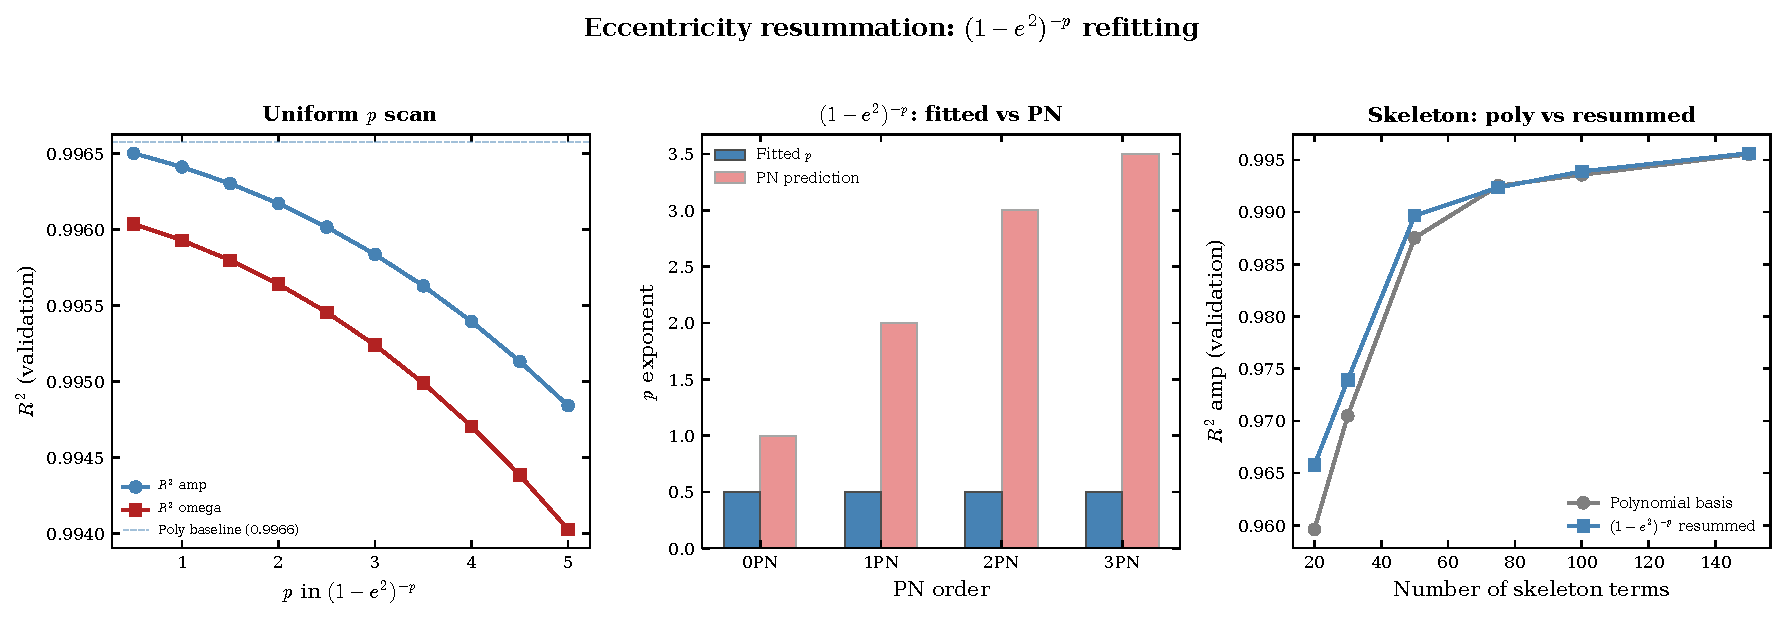
\includegraphics[width=\textwidth]{resum_ecc_refit.pdf}
\caption{$(1-e^2)^{-p}$ refitting results. \textbf{Left}: $R^2$ vs uniform $p$ --- best at $p = 0.5$. \textbf{Centre}: fitted $p$ per PN order (blue) vs PN predictions (red). \textbf{Right}: skeleton scan on polynomial vs resummed basis.}
\label{fig:resum_refit}
\end{figure}

The full set of 75 coefficients for both $\dxamp$ and $\dxomg$ is tabulated in the supplementary file \texttt{compact\_coefficients.json}.

%======================================================================
\section{Summary of Physical Content}
\label{sec:summary}
%======================================================================

\begin{enumerate}[nosep]
\item The PN ansatz ($|h_{22}^{\rm ecc}| - 1$ at 0PN + 1PN) provides the \textbf{Keplerian backbone}: the dominant $e\cos\zeta/(1-e^2)$ modulation with first-order relativistic corrections.

\item The Ridge residual primarily adds:
\begin{itemize}[nosep]
\item[$\triangleright$] \textbf{$\sin\zeta$ phase content} ($\sim$40\% of residual): the imaginary part of $h_{22}^{\rm ecc}$ that is lost when taking the absolute value. Represents orbital phase modulation at the pericenter/apocenter asymmetry.

\item[$\triangleright$] \textbf{Spin-orbit and spin-spin corrections} ($\sim$55\% via $\chiS$, $\chiA$): entering at 1.5PN, approximated in the integer-power basis as combinations of $x^1\chi$ and $x^2\chi$ (the true scaling is $x^{3/2}\chi$).

\item[$\triangleright$] \textbf{Higher PN orders}: 2PN ($x^2$, $\nu^2$-dependent), 2.5PN ($x^{5/2}$, approximated by $x^3$), and 1.5PN tail effects ($\pi x^{3/2}$, logarithmic terms).

\item[$\triangleright$] \textbf{Resummation of $(1-e^2)^{-p}$}: the eccentricity-enhanced PN denominators are reconstructed through $e^3$--$e^5$ terms.
\end{itemize}

\item The amplitude--frequency relation $\xomg \approx \xamp/B$ holds with $B_{\rm eff} \approx 0.78$ (non-spin) and $B_{\rm eff} \approx 0.69$ (spin), compared to the gwNRXHME prediction $B = 0.9$ (Fig.~\ref{fig:rel_iii}). Spin-orbit coupling modifies the frequency more than the amplitude.

\item \textbf{Compactification} (Sections~\ref{sec:compact_results}--\ref{sec:skeleton}): Two levels of compression are achieved:
\begin{itemize}[nosep]
\item Fourier truncation to $k \leq 3$: 2955 $\to$ \textbf{1379 parameters with no accuracy loss} ($R^2 = 0.9966$ preserved).
\item Skeleton-75: importance-based selection + refitting yields \textbf{75 terms with $R^2 = 0.9925$} --- a 40$\times$ compression. The resulting formula (Eq.~\ref{eq:compact_physical}) is analytically interpretable and cleanly separates into non-spin ($\sin\zeta$ phase content), spin-orbit ($\chiS$, $\chiA$ at 1.5PN), and subdominant $\cos\zeta$ corrections.
\end{itemize}
\end{enumerate}

%======================================================================
\section{Recommended Next Steps}
\label{sec:next}
%======================================================================

\begin{enumerate}[nosep]
\item[\checkmark] \textbf{Fourier diagnostic}: Completed (Fig.~\ref{fig:fourier_diag}, Table~\ref{tab:fourier_summary}). Geometric decay rates $r \approx 0.55$--$0.77$; $k = 1$ dominates overwhelmingly.

\item[\checkmark] \textbf{Fourier truncation + Pad\'e}: Completed (Table~\ref{tab:trunc_r2}, Figs.~\ref{fig:trunc_acc},~\ref{fig:pade_comp}). Truncation to $k \leq 3$ preserves full accuracy with 53\% parameter reduction.

\item[\checkmark] \textbf{$(1-e^2)^{-p}$ extraction}: Completed (Fig.~\ref{fig:resum_p}). Consistent with PN expectations at 1PN ($p \approx 2$); higher PN sectors have weak eccentricity enhancement.

\item[\checkmark] \textbf{PN comparison + spin decomposition}: Completed (Figs.~\ref{fig:pn_decomp}--\ref{fig:spin_contrib}). Residual's $\sin\zeta$ content and spin-orbit structure confirmed.

\item[\checkmark] \textbf{Relation III analysis}: Completed (Fig.~\ref{fig:rel_iii}). Effective $B_{\rm eff} = 0.78$ (non-spin), $0.69$ (spin).

\item[\checkmark] \textbf{Skeleton compactification}: Completed (Section~\ref{sec:skeleton}). Importance-ranked selection + refit: 75 terms achieve $R^2 = 0.9925$ (40$\times$ compression). Clean separation into non-spin $\sin\zeta$ (39 terms), $\chiS$ spin-orbit (18), $\chiA$ spin-orbit (18). Compact formula in Eq.~\eqref{eq:compact_physical}; full coefficients in \texttt{compact\_coefficients.json}.

\item[$\circ$] \textbf{Spin-augmented ansatz}: Extend $h_{22}^{\rm ecc}$ to include the leading 1.5PN spin-orbit term from \texttt{EOB\_modes.dat.m}, absorbing the largest 55\% of the residual into the known physics.

\item[$\circ$] \textbf{Half-integer basis}: Add $x^{3/2}$ and $x^{5/2}$ to the basis to directly capture 1.5PN and 2.5PN scaling, consolidating the coefficient pairs that currently split across $x^1$ and $x^2$.

\item[\checkmark] \textbf{$(1-e^2)^{-p}$ refitting}: Completed (\texttt{resum\_ecc.py}, Fig.~\texttt{resum\_ecc\_refit.pdf}).
Refitted the full $k\!\leq\!3$ basis with explicit $(1-e^2)^{-p}$ denominators at each PN order.
Scanned $p \in [0.5, 5.0]$ uniformly and independently per PN sector. \textbf{Key results}:
\begin{itemize}[nosep]
  \item All PN orders prefer $p = 0.5$, \emph{not} the expected PN values ($p = 1, 2, 3, 3.5$).
  This is because the polynomial $e^1$--$e^5$ basis already captures the $(1-e^2)^{-p}$ Taylor expansion within the training range $e \in [0, 0.5]$, so the residual prefers minimal eccentricity enhancement.
  \item $R^2$ change is negligible: $-0.007\%$ (amp), $-0.009\%$ (omega).
  \item LIGO mismatch is \textbf{identical}: polynomial median $= 5.95 \times 10^{-4}$ vs resummed $= 5.95 \times 10^{-4}$ (750 pts, all $M_{\rm tot}$); p90 agreement to 3 significant figures.
  \item Skeleton scan (resummed basis, top-75 refit): $R^2_{\rm amp} = 0.9923$, comparable to polynomial skeleton ($0.9925$).
  \item \textbf{Conclusion}: Within $e_0 \leq 0.5$, the polynomial and resummed bases are effectively equivalent. The $(1-e^2)^{-p}$ resummation becomes valuable only for \emph{extrapolation} to $e > 0.5$ or for \emph{interpretive display} (connecting to known PN structure).
\end{itemize}
\end{enumerate}

\end{document}
